\documentclass[11pt]{article}

\usepackage[hyperfootnotes=false]{hyperref}                                    
\usepackage{amsmath,amsthm,amssymb}      
\usepackage{titlesec}                                                         
\usepackage{bm}        
\usepackage{cprotect}                                
%\usepackage{savetrees} 
\usepackage{bbold}
\usepackage{abstract}

\usepackage{tikz}
\usetikzlibrary{arrows}
                                          
\usepackage{graphicx}                                      
\graphicspath{{../figures/}, {../figures/growthrates/}, {../figures/correlations/}, {../python/Hamiltonian/figures/}}

\usepackage[sorting=none, url=false]{biblatex}
\bibliography{bib.bib}

% Formatting
\usepackage{indentfirst}
\usepackage{geometry}  
\geometry{margin=1in}       
\geometry{lmargin=1.5in} 
\titleformat{\subsection}
{\normalfont\large\bfseries}{\thesubsection}{1em}{}
\renewcommand{\baselinestretch}{1.1}

\renewcommand{\bf}{\mathbf}
\renewcommand{\cal}{\mathcal}
\newcommand{\pd}[2]{\frac{\partial #1}{\partial #2}}
\newcommand{\pdn}[3]{\frac{\partial^{#3} #1}{\partial #2^{#3}}}
\newcommand{\pdop}[1]{\frac{\partial}{\partial #1}}
\newcommand{\nd}[2]{\frac{d #1}{d #2}}
\newcommand{\ndn}[3]{\frac{d^{#3} #1}{d #2^{#3}}}
\newcommand{\ndop}[1]{\frac{d}{d #1}}
\newcommand{\dt}{\frac{d}{dt}}
\newcommand{\grad}{\bm\nabla}
\newcommand{\cross}{\times}
\newcommand{\curl}{\grad\cross}
\newcommand{\imp}{\Longrightarrow\quad}
\newcommand{\abs}[1]{\left|#1\right|}
\newcommand{\half}{\frac{1}{2}}
\newcommand{\third}{\frac{1}{3}}
\renewcommand{\th}[1]{\frac{1}{#1}}
\renewcommand{\k}{4\pi\epsilon_0}
\newcommand{\eps}{\epsilon_0}
\newcommand{\intt}{\int_{t_1}^{t_2}}
\newcommand{\inti}{\int_{-\infty}^{+\infty}}
\newcommand{\ex}[1]{\left\langle #1 \right\rangle}
\newcommand{\oom}[1]{\times 10^{#1}}
\renewcommand{\d}{\delta}
\newcommand{\e}{\text{e}}
\renewcommand{\l}{\ell}
\newcommand{\om}{\omega}
\newcommand{\h}{\hbar}
\newcommand{\ket}[1]{\left|#1\right\rangle}
\newcommand{\bra}[1]{\left\langle#1\right|}
\newcommand{\braket}[2]{\left\langle#1\middle|#2\right\rangle}
\newcommand{\brakett}[3]{\left\langle#1\middle|#2\middle|#3\right\rangle}
\newcommand{\nn}{\nonumber\\}

\DeclareMathOperator{\Tr}{Tr}
\let\Re\relax
\DeclareMathOperator{\Re}{Re}

\begin{document}
	
\pagenumbering{Roman}
%{\setstretch{1.5}
\vspace*{.2in}
\begin{center}
	\huge{\textbf{Operator and Entanglement Dynamics \\
			        in Asymmetric Quantum Systems}}
\end{center}
\vspace{.6in}
\sc
\begin{center}
	\LARGE{Charles Nicholas Stahl}
\end{center}
\vspace{.6in}
\begin{center}
\today
\end{center}
\vspace{.6in}
\begin{center}
	{\Large Advised by Professor David Huse} \\
	Second Reader: Professor Shivaji Sondhi
\end{center}
\vspace{.6in}
\begin{center}
	Submitted in partial fulfillment \\
	of the Requirements for the \\
	Degree of Bachelor of Arts
\end{center}
}
\newpage

\begin{abstract}
	Thermalization is an important aspect in quantum physics from condensed matter to black holes. It allows initially local information to be spread and hidden throughout a system. This spreading happens at a finite speed, and can be quantified using the butterfly velocity $v_B$ or the entanglement velocity $v_E$. Although many sources have explored these sources, fewer explore the ratio $v_E/v_B$, and little work has been in describing asymmetric butterfly velocities. In this thesis we find both a time-independent system and a quantum circuit with different butterfly velocities in either direction, which we call $v_{B\pm}$. Although in the Hamiltonian system the two velocities are still close in magnitude, the ratio $v_{B+}/v_{B-}$ can be made arbitrarily large in the circuit model.\blfootnote{I pledge my honor that this paper represents my own work in accordance with University regulations.}
\end{abstract}

\newpage

\section*{Acknowledgments}

\newpage

\tableofcontents
\pagenumbering{arabic}
\input{introduction}
\section{Operator Spreading in Time-Independent Hamiltonian Systems} \label{sec:opsp}

Just do all intro here, and then decide later what to put into the circuit section

Thermalization 
  vs localization 
  happens by spreading information
  mention that this is how information loss happens

Discuss information movement in Time-Independent Hamiltonian systems
  Find a source for this
  Ideally introduce OTOC and Pauli end weight here
  Also entanglement possibly
  What is the relationship between entropy and OTOC?
  Argument about extremal slope
    From Nahum: stairs to separate $v_B$ and $v_E$
    

For now use Jonay paper, but hopefully find another. Could use Keyserlingk but it would be nice to save that for the discussion of random unitary dynamics.

Although most sources consider symmetric dynamics [CITE] this is not a requirement. Find the Nahum paper that discusses asymmetric systems.
%\section{Dynamics in an Asymmetric Hamiltonian} \label{sec:asymham}

\subsection{3-Site Hamiltonian} \emph{} \label{sub:hamiltonian}

Instead of a Floquet or quantum circuit system, we can consider one with a time-independent Hamiltonian, for a finite number of dimensions at each site. We can choose a Hamiltonian based on how uneven its dynamics are. For example, the three-site swap $S_{123}$ is a unitary operator such that 
\begin{align}
S_{123}\psi_1\psi_2\psi_3 =\psi_2\psi_3\psi_1, \label{eqn:condition}
\end{align}
where the position of the wavefunction denotes the site on which it sits. 

One way to build the three site swap gate is in a Floquet system, out of two site swap gates $S_{123} = S_{23}S_{12}$. However it is also possible to build it out of a time-independent Hamiltonian, so that $U(1) = \e^{-iH_3} = S_{123}$. This is possible by either taking the matrix-log of $S_{123}$ or by considering the eigenstates and corresponding eigenvalues. 

For a spin-$\half$ system, there will be 8 states, which can be decomposed into a spin-$\frac{3}{2}$ subspace with 4 states and 2 spin-$\half$ subspaces with 2 states each. The eigenstates will be states in which individual particle states differ only by phases. There are four states that should not change in time and therefore have 0 energy. Before normalization these are
\begin{align}
\ket{000},\quad \ket{100}+\ket{010}+\ket{001},\nn
\ket{111},\quad \ket{011}+\ket{101}+\ket{110}.\label{eqn:zero}
\end{align}
Of the four other states, two should have positive energy and two should have negative energy. Since $U(3)=1$, their energies should be $E_\pm = \pm\frac{2\pi}{3}$ so they pick up a phase $\phi_\pm =\e^{-iE_\pm} = \e^{\mp i\frac{2\pi}{3}}$. Using condition~\ref{eqn:condition}, we can show that the positive energy states are
\begin{align}
&\ket{100} + \phi_-\ket{010} + \phi_+\ket{001},\nn
&\ket{011} + \phi_-\ket{101} + \phi_+\ket{110},\label{eqn:plus}
\end{align}
while the negative energy states are 
\begin{align}
&\ket{100} + \phi_+\ket{010} + \phi_-\ket{001},\nn
&\ket{011} + \phi_+\ket{101} + \phi_-\ket{110}.\label{eqn:minus}
\end{align}

In matrix notation, with basis states $\ket{000},\,\ket{001},\,\ket{010},$ etc, the hamiltonian is 
\begin{align}
H_3 = T\; \text{diag}(0,0,0,0,E_+,E_+,E_-,E_-)\; T^\dag,
\end{align}
where $T$ is the transformation matrix suggested by~\ref{eqn:zero}, \ref{eqn:plus}, and~\ref{eqn:minus},
\begin{align}
T = \th{\sqrt{3}}\begin{bmatrix}
\sqrt{3} & 0 & 0 & 0        & 0      & 0      & 0      & 0      \\
0        & 1 & 0 & 0        & \phi_+ & 0      & \phi_- & 0      \\
0        & 1 & 0 & 0        & \phi_- & 0      & \phi_+ & 0      \\
0        & 0 & 1 & 0        & 0      & 1      & 0      & 1      \\
0        & 1 & 0 & 0        & 1      & 0      & 1      & 0      \\
0        & 0 & 1 & 0        & 0      & \phi_- & 0      & \phi_+ \\
0        & 0 & 1 & 0        & 0      & \phi_+ & 0      & \phi_- \\
0        & 0 & 0 & \sqrt{3} & 0      & 0      & 0      & 0
\end{bmatrix}
\end{align}
Altogether
\begin{align}
H_3 = \frac{2\pi i}{\sqrt{3}}\begin{bmatrix}
0 & 0  & 0  & 0  & 0  & 0  & 0  & 0 \\
0 & 0  & 1  & 0  & -1 & 0  & 0  & 0 \\
0 & -1 & 0  & 0  & 1  & 0  & 0  & 0 \\
0 & 0  & 0  & 0  & 0  & -1 & 1  & 0 \\
0 & 1  & -1 & 0  & 0  & 0  & 0  & 0 \\
0 & 0  & 0  & 1  & 0  & 0  & -1 & 0 \\
0 & 0  & 0  & -1 & 0  & 1  & 0  & 0 \\
0 & 0  & 0  & 0  & 0  & 0  & 0  & 0 \\
\end{bmatrix}
\end{align}

This hamiltonian should be symmetric under a simultaneous rotation of all three spins, so that it can be written as $H_3(\bm{\sigma}_1,\,\bm{\sigma}_2 ,\,\bm{\sigma}_3)$. It should be antisymmetric under the interchange of any two spins (equivalent to reversing the direction of propagation). The only function of three vectors that has this property is the triple product $H_3= \bm{\sigma}_1\cdot\left(\bm{\sigma}_2 \times\bm{\sigma}_3\right)$.

%Note that this is equivalent to
%\begin{align}
%H &= \bm{\sigma}_1\cdot\left(\bm{\sigma}_2 \times\bm{\sigma}_3\right) \nn
% &= \sigma_{1,1}\otimes\sigma_{2,2}\otimes{\sigma}_{3,3} - {\sigma}_{1,1}
%	\otimes\sigma_{2,3}\otimes\sigma_{3,2} + \sigma_{1,2}\otimes{\sigma}_{2,3} \otimes {\sigma}_{3,1}-\cdots
%\end{align}

Exponentiating the hamiltonian gives the time evolution operator for one time step
\begin{align}
U(1) = \e^{-iH_3} = \begin{bmatrix}
1 & 0 & 0 & 0 & 0 & 0 & 0 & 0 \\
0 & 0 & 1 & 0 & 0 & 0 & 0 & 0 \\
0 & 0 & 0 & 0 & 1 & 0 & 0 & 0 \\
0 & 0 & 0 & 0 & 0 & 0 & 1 & 0 \\
0 & 1 & 0 & 0 & 0 & 0 & 0 & 0 \\
0 & 0 & 0 & 1 & 0 & 0 & 0 & 0 \\
0 & 0 & 0 & 0 & 0 & 1 & 0 & 0 \\
0 & 0 & 0 & 0 & 0 & 0 & 0 & 1
\end{bmatrix}
\end{align}
This has the properties of of condition~\ref{eqn:condition}. Furthermore, application three times gives $U(3) = 1$. The hamiltonian commutes with the total spin-Z operator $S_Z = \text{diag}(\frac{3}{2}, \frac{1}{2}, \frac{1}{2}, -\frac{1}{2}, \frac{1}{2}, -\frac{1}{2}, -\frac{1}{2}, -\frac{3}{2})$ so total spin-Z is conserved. It also commutes with the other components of spin and therefore also total spin $S^2$.

If the system starts in a computational basis state, for example $\ket{100}$, the coefficients for the other states with equal total spin-Z will both change from 0 before the states becomes $\ket{010}$ at time 1, as in figure~\ref{fig:timeevol}.
\begin{figure}
	\centering
	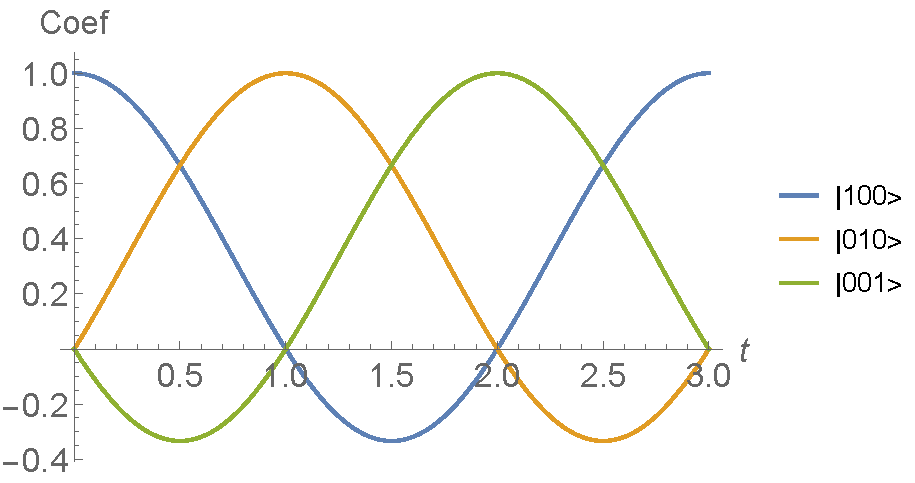
\includegraphics[width=.5\textwidth]{timeevol}
	\caption{Evolution of coefficients if the system starts in state $\ket{100}$.}
	\label{fig:timeevol}
\end{figure}

\subsection{Multi-Site Hamiltonian} \emph{}\label{sub:multistate}

\subsubsection{Construction} \label{subsub:construction} \emph{}

There are multiple ways to extend this hamiltonian to a chain of $L= 2n+1$ spins. Like building $S_{123}$ out of two-site swaps we can treat the larger system as a Floquet system, successively applying $H_3$ to each triplet of spins. We can define a similar hamiltonian by putting the 3-site hamiltonian simultaneously on sites 1-3, sites 3-5, etc. For $n=2$, this is
\begin{align}
H_5 = H_3\otimes\mathbb{I}_2 + \mathbb{I}_2\otimes H_3.
\end{align} 
This hamiltonian still preserves each component of total spin. 

Starting in $\ket{00001}$, the coefficients follow the pattern of figure~\ref{fig:timeevol5}. At first the evolution is similar to the $n=1$ case, with $\ket{10000}$ and then $\ket{01000}$ reaching near maximal. The coefficient of $\ket{00001}$ is 
\begin{align}
\frac{1}{10} \left(3 \cos \left(\frac{2}{3} \sqrt{\frac{5}{3}} \pi  t\right)+5 \cos \left(\frac{2 \pi  t}{3 \sqrt{3}}\right)+2\right)
\end{align} 
which is shown in figure~\ref{fig:onecoef}. Although it appears to be quasi-periodic, it cannot ever reach 1 for $t\ne 0$ or be truly periodic because its time coefficients are not rationally related.

\begin{figure}
	\centering
	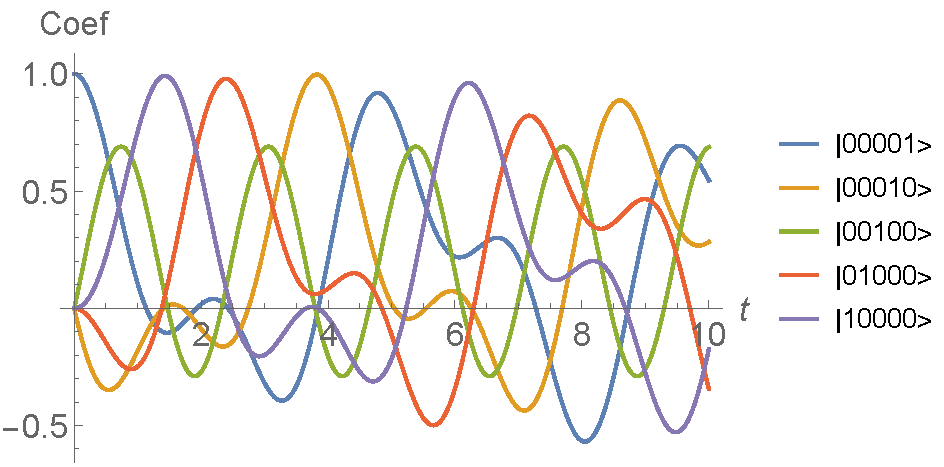
\includegraphics[width=.5\textwidth]{timeevol5}
	\caption{Evolution of coefficients if the system starts in state $\ket{00001}$.}
	\label{fig:timeevol5}
\end{figure}

\begin{figure}
	\centering
	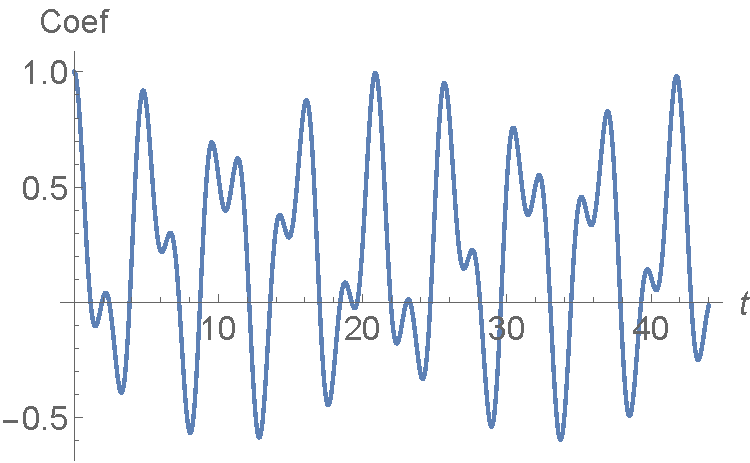
\includegraphics[width=.5\textwidth]{onecoef}
	\caption{Coefficient for $\ket{00001}$ when that is the starting state.}
	\label{fig:onecoef}
\end{figure}

%The coefficient for $\ket{00100}$ does not fit the pattern. It does not reach maximum at the right time and it does have a periodic structure. Furthermore, when the starting state is $\ket{00010}$ the problematic state is still $\ket{00100}$, probably because of the chaining mechanism. When the starting state is $\ket{00100}$ the coefficients for $\ket{10000}$ and $\ket{00001}$ always vanish. The next chaining method to try will be to have $2n$ spins, and to have the first spin complete the last trio.

\subsubsection{Pauli String Weight} \label{subsub:operator_dynamics} \emph{} 

We can study the operator dynamics of this system by extending to large $L$ and evolving operators that are identities on all sites except one end. Since the hamiltonian is SO(3) symmetric, it does not matter if the perturbation is $X$, $Y$, or $Z$. For convenience, we will use $Z$. We can then study the weight of strings that end at each site $i$, $W(t; i)$.

For the forward-propagating wave, with $A(t=0) = Z_0 = Z\otimes \mathbb{I} \otimes \mathbb{I} \cdots$, the weight starts on site 0 and peaks at even sites. The successive peaks fall off in size but dominate the Pauli strings until the last site takes over (figure~\ref{fig:L11end3n20front}). This is possibly because 

For the backward-propagating waves $(A(t=0)=Z_{L-1})$, the initial decaying signal is more difficult to make out but still present. It is dominated by a large weight of sites that start on site 9 around $t=1$. By $t = 3$ the first site has started to dominate the Pauli weights.

\begin{figure}
	\centering
	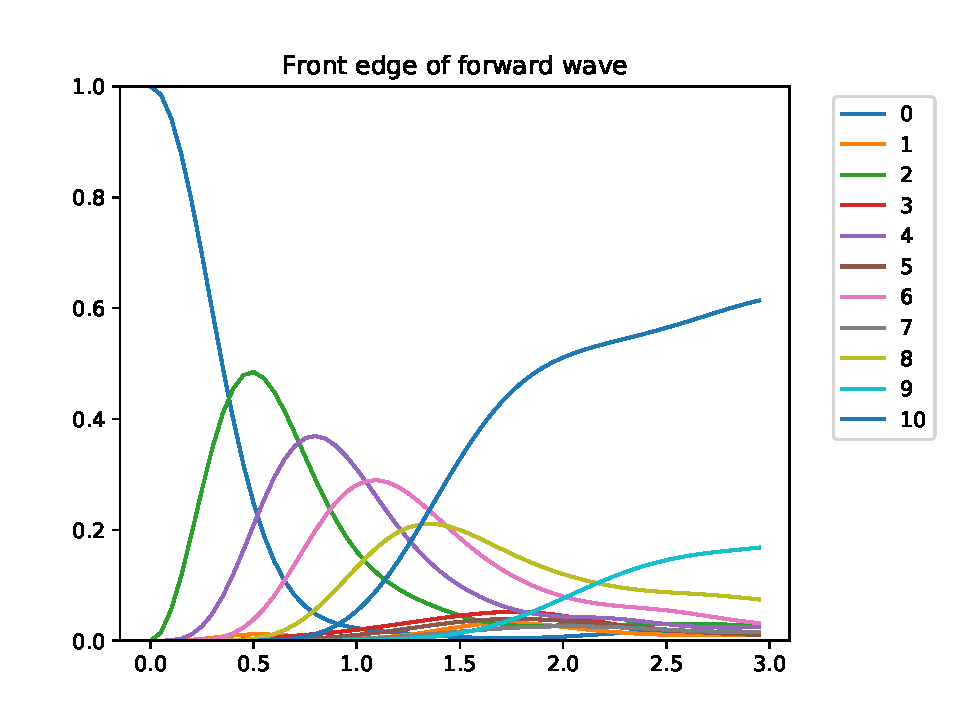
\includegraphics[width=.7\textwidth]{L11end3n20front}
	\caption{Weight of operators that end on site $i$.}
	\label{fig:L11end3n20front}
\end{figure}
\begin{figure}
	\centering
	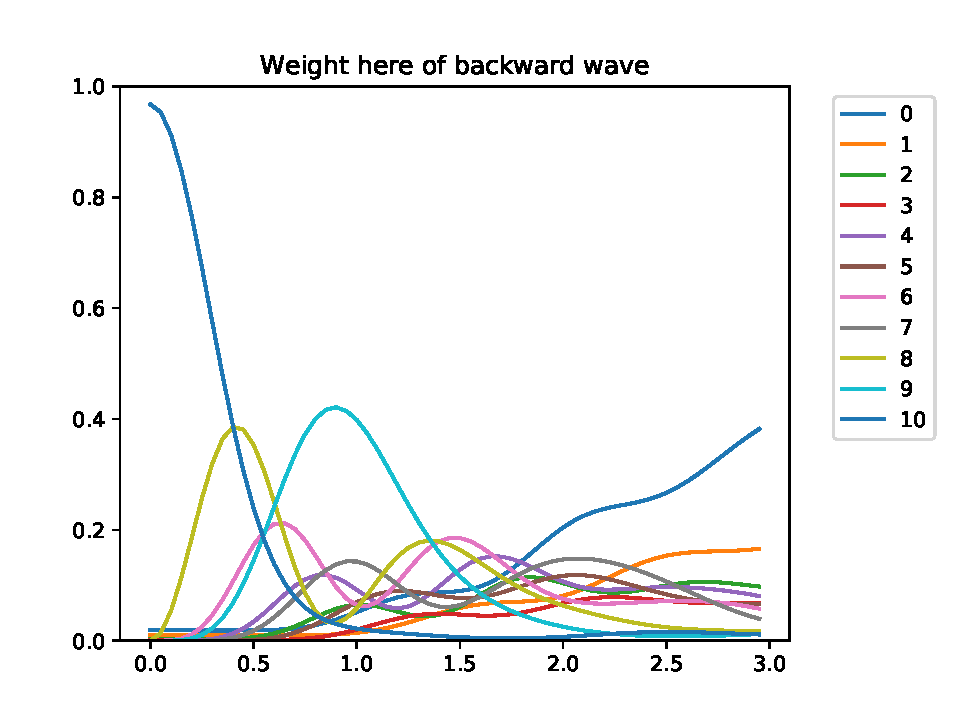
\includegraphics[width=.7\textwidth]{L11end3n20back}
	\caption{Weight of operators that begin on site $i$.}
	\label{fig:L11end3n20back}
\end{figure}

The initial behavior also matches the $L=9$ case. For forward propagation the initial behavior is $W(t;i) = a\e^{bt}$ with $a,b$ given by\dots Figure~\ref{fig:L11end1n60fore} shows this behavior, while figure~\ref{fig:L11end1n60back} shows the analogous behavior for the backward propagating wave. 

\begin{figure}
	\centering
	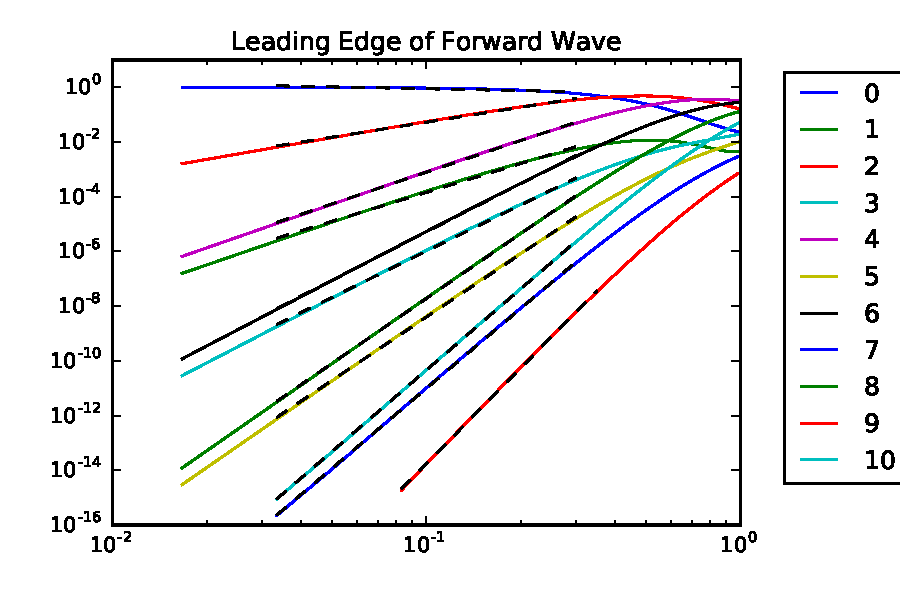
\includegraphics[width=.7\textwidth]{L11end1n60fore}
	\caption{Early-time leading edge weights for forward propagating wave.}
	\label{fig:L11end1n60fore}
\end{figure}
\begin{figure}
	\centering
	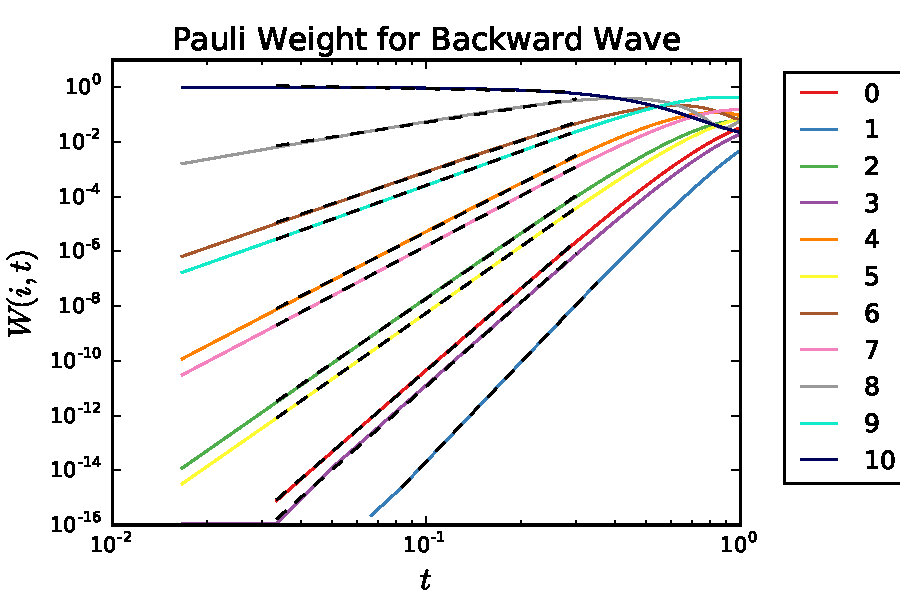
\includegraphics[width=.7\textwidth]{L11end1n60back}
	\caption{Early-time leading edge weights for backward propagating wave.}
	\label{fig:L11end1n60back}
\end{figure}

Here the relevant numbers are\dots
Again, the exponents for even and odd sites increase by one within each group. Pairs of sites separated by 3 are also divergent in the forward case while convergent in the backward case.
%\section{Entanglement and Operator Spreading in Quantum Circuits} \label{sec:circuits}

One drawback to studying systems with time-independent Hamiltonians is that their dynamics are constrained by their conservation laws~\cite{Jonay18}. Systems with no conservation laws would not have these constraints. Quantum circuits have no explicit Hamiltonian, but rather evolve unitarily at discrete time steps, making them ideal for studying unconstrained dynamics. Furthermore, while numerical simulation of the Hamiltonian system is limited to small systems with large finite size effects, quantum circuits can have solvable dynamics that can be efficiently simulated.

The circuits provide solvable systems in certain limits, after averaging over circuit architecture. In this limit, which will be discussed later in this section, it is easier to discuss information dynamics in terms of entanglement entropy rather than operator spreading. This is not to say that operator spreading does not apply in circuits, or that entanglement dynamics do not apply to Hamiltonian systems. Rather, this is an easier tool to use for these systems.

In this section we first introduce bitartite entanglement entropy and the constraints it must satisfy. We then discuss the construction of quantum circuits, and the behavior of the entanglement entropy in these circuits. We show that it is possible to calculate $v_B$ entirely from the entanglement entropy, and that this velocity is the same as $v_B$ calculated from operator spreading.

\subsection{Entanglement Entropy} \label{sub:intro}

Quantum entanglement has applications to branches of physics from high energy and quantum information theory to experimental studies of cold atomic gases. Although entanglement is so widely studied, its dynamics are less well understood. The dynamics of the entanglement are closely related to the speed at which information travels or spreads. 

Let us briefly review entanglement in composite systems. First assume the full system $AB$ can be decomposed into subsystems $A$ and $B$, and $AB$ is in the pure state $\ket{\Psi}_{{AB}}$. In the spin chains considered here, the chain is often divided such that $A$ is all spins on one side of a cut and $B$ is all spins on the other side. Another common decomposition is having $A$ be all spins between two cuts, and $B$ being all other spins. If the states of $A$ and $B$ are entangled it is impossible to write $\ket{\Psi}_{AB} = \ket{\psi_A}_A \ket{\psi_B}_B$. If this is possible then $\ket{\Psi_{{AB}}}$ is called a product state. Subscripts on kets represent the space that the ket lives in, but this is clear from the name of the state (uppercase for the full state, subscripts otherwise) so we will drop the outside subscripts.

We can assess the amount of entanglement by looking at the density matrix $\rho_{AB} = \ket{\Psi}\bra{\Psi}$. All density matrices satisfy $\Tr \rho = 1$. Generic pure state density matrices further satisfy 
\begin{align}
\Tr \rho^2 = \Tr\ket{\psi}\bra{\psi}\ket{\psi}\bra{\psi} = \Tr\ket{\psi}\bra{\psi} = 1.
\end{align}
We can further construct the reduced density matrices $\rho_A$ and $\rho_B$ as the full density matrix $\rho_{AB}$ traced over subsystem $B$ and $A$, respectively. If $\ket{\Psi}$ is a product state, the reduced density matrices are $\rho_A = \ket{\psi_A}\bra{\psi_A}$, etc. However, if the states are entangled the reduced density matrices do not have such a nice form. They will still have trace 1, but $\Tr\rho^2<1$ for a mixed state.

A maximally entangled state will be of the form
\begin{align}
\ket{\Psi} = \sum_i^N\th{\sqrt{N}}\ket{\psi_{A,i}}\ket{\psi_{B,i}},
\end{align}
where $N$ is the dimension of the larger of the two Hilbert spaces and $i$ labels orthogonal states. $\Tr\rho_{AB}^2=1$ because the full state is pure. The reduced density matrices are
\begin{align}
\rho_A = \sum_i^N\th{N}\ket{\psi_{A,i}}\bra{\psi_{A,i}},
\end{align}
with $\Tr\rho_A^2 = \sum_i\th{N^2}=\th{N}$, with similar results for $B$. This provides the constraints $\th{N}\le\Tr\rho^2\le 1$. 

Bipartite entanglement entropy provides a more general way to quantify the entanglement and is defined as the quantum entropy of one of the reduced density matrices. As long as the full state is pure, this is equivalent for either subsystem. There are multiple quantum entropies. The $n$th Renyi entropy of density matrix $\rho$ is 
\begin{align}
S_n = \th{1-n}\log\left(\Tr\rho^n\right). \label{eqn:renyi}
\end{align}
In the limit $n\to1$ this becomes the von Neumann entropy 
\begin{align}
S_{vN} &= \th{1-(1+\epsilon)}\log\left(\Tr\rho^{1+\epsilon}\right) \nn
&= -\frac{1}{\epsilon}\log \Tr \rho \rho^{\epsilon}\nn
&= -\th{\epsilon}\log\Tr\rho\left(1+\epsilon\rho\right) \nn
&= -\Tr\rho\log\rho,
\end{align}
the analogue of the classical Shannon entropy. The calculation uses the small $x$ expansions of $a^x$ and $\log(1+x)$. All Renyi entropies are maximized by maximally mixed states, with entropy $N\log q$ for $N$-site systems with $q$-dimensional Hilbert spaces at each site. They are also minimized by pure states, which have entropy 0.

For the spin chain, we can define many different subsystems, each with a corresponding entanglement entropy. The following description is largely taken from~\cite{Nahum2017}. Consider a spin chain of N sites with dimension $q$. Sites are labeled by $i=1,\dots N$, while the bonds between sites are labeled by $x = 1,\dots N-1$. After cutting the system at bond $x$, define the entropy across this cut as the bipartite entanglement entropy of all sites to the right of $x$. If the whole chain is in a pure state, this is equal to the bipartite entanglement entropy of all sites to the left of $x$.

We can define a function $S(x) = -\Tr\rho_x\log\rho_x$ where $\rho_x$ is the density matrix of the system with all sites left of $x$ traced out. As long as the full system is in a pure state, this is the von Neumann entanglement entropy of the two subsystems divided by the bond at $x$. For convenience logarithms are taken base $q$. $S(x)$ will observe constraints not already made clear due to the fact that subsystems defined by adjacent $x$ have heavy overlap.

Classically, for an arbitrary system decomposable into subsystems $A$ and $B$, the entropies satisfy $\max(S(A), S(B)) \leq S(AB)\leq S(A) + S(B)$. In quantum mechanics, this is replaced by the subadditivity of the von Neumann entropy 
\begin{align}
\left|S(A)-S(B)\right| \leq S(AB)\leq S(A) + S(B). \label{eqn:subadd}
\end{align}
If we take subsystem $A$ to be the single site between cuts $x$ and $x+1$ and subsystem $B$ to be all sites right of $x+1$, this becomes
\begin{align}
\left|S_1 - S(x+1)\right| \leq S(x) \leq S_1 + S(x+1),
\end{align}
where $S_1$ denotes the entropy of the single site between cuts $x$ and $x+1$. After some rearranging this can be written $\left|S(x+1) - S(x)\right| \leq S_1$. However, since the single site is $q$ dimensional, $S_1 \leq \log_q q = 1$, explaining the use of $q$ for the base. The preceding arguments taken together give the constraint
\begin{align}
\left|S(x+1) - S(x)\right| \leq 1. \label{eqn:offbyone}
\end{align}

A finite system has $S(x)$ pinned at its endpoint, because the entanglement entropy of a single site is bounded by 1. Then the maximally entangled state has $S(x) = \min\{x,L-x\}$. As the entanglement approaches this value it takes forms as in Fig.~\ref{fig:Tower}.
\begin{figure}
	\centering
	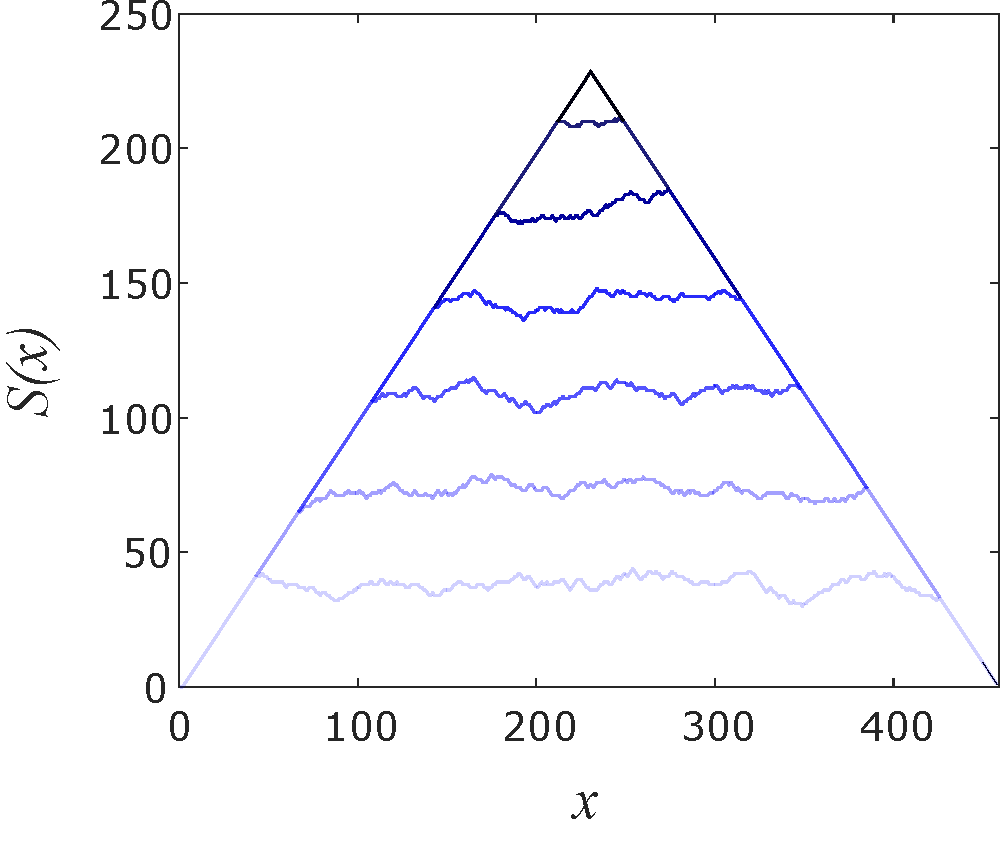
\includegraphics[width=.5\linewidth]{Tower}
	\caption{\textbf{Bitartite entanglement entropy at different times,} ($t = 340$, 690, 1024, 1365, 1707, 2048 and 4096). This data comes from a circuit model, but the behavior is believed to be general. Figure from~\cite{Nahum2017}.}
	\label{fig:Tower}
\end{figure}
The flat section has a constant growth rate $\pd{S(x,t)}{t}$ so the border position $y$ moves at a constant speed defined by the growth rate and the slope. Since the maximal slope is $\pd{S(x,t)}{x}=1$, this velocity is
\begin{align}
\pd{y}{t} = \pd{S}{t}\left(\pd{S}{x}\right)^{-1} = \pd{S}{t} = v_E. 
\label{eqn:vE}
\end{align}
This entanglement speed is equivalent to the entanglement growth rate, under certain assumptions not mentioned here. This calculation is repeated more generally and in more detail in Sec.~\ref{sub:coarse}.

Refs.~\cite{Keyserlingk, Jonay17, Jonay18, Nahum2017} discuss the speed of entanglement in brickwork models using the OTOC and operator density. Reference~\cite{Zhou2017} quantifies the scrambling using the operator entanglement entropy opEE of the time evolution operator.

\subsection{Circuit Architectures} \label{sub:arch}

Like the earlier systems, quantum circuits consist of chains of Hilbert spaces. Instead of evolving under a time-independent Hamiltonian, they evolve with unitary operators, called gates, at discrete times. If a gate acts on a site at time $t$ it is said to `fall' on that site. Simple circuits only contain 2-site gates which act on the product of Hilbert spaces at adjacent sites. There is a possibility of confusion regarding the term ``operator": the ``unitary operator," ``unitary gate," or just ``gate" will be the time evolution operator of the circuit, while ``operator" without qualification will refer to the observable that is evolving in time.

We could study the dynamics of a single circuit, in analogy with the single Hamiltonian studied in the previous section. However, it is also instructive to look at ensembles of circuits, with some type of randomness. This section presents two sources of randomness, the choice of gates and their locations in the circuit.

%References~\cite{Keyserlingk} and~\cite{Nahum2017} both discuss circuits of this type. Both discuss random circuits, although with different sources of randomness. 
One source is the unitary operator chosen at each site at each time. Different gates result in different architectures. 
If the Hilbert space at each site is $q$ dimensional, the space of 2-site unitary matrices is $q^2\times q^2$ dimensional. To find representative behavior, each circuit is made by drawing gates from some distribution. The circuits can then be averaged over these choices. A common choice is the Haar distribution, which is invariant to rotations in the space of 2-site operators. Since these act on a $q^2$-dimensional Hilbert space, there are $q^4$ independent operators, including one trivial operator (the identity). 

Another source of randomness is the placement of the gates. The ``brickwork" model~\cite{Keyserlingk} uses a deterministic architecture, in which at odd times there is a gate to the right of every odd site, while for even times there is a gate to the right of every even site. Figure~\ref{fig:brickcircuit} shows an example. The ``random" architecture~\cite{Nahum2017} chooses a random site for a single gate at each time step $t = n/\gamma$, where $\gamma$ is the gate rate and $n$ is an integer. The placement is then averaged over. 

\begin{figure}
	\centering
	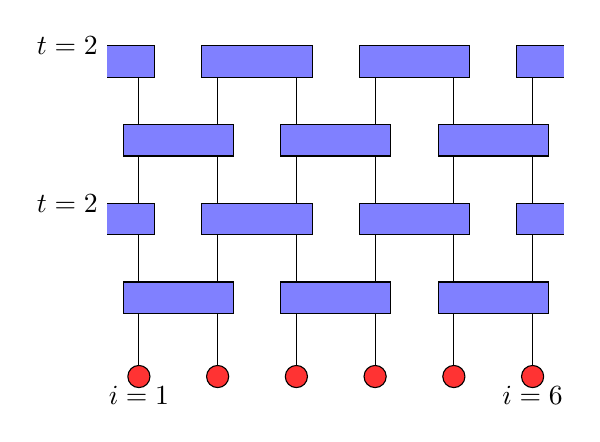
\begin{tikzpicture}[scale = 1]
\draw (0,0) node[below]{$i=1$} -- (0,4);
\filldraw[color=black, fill=red!80] (0,0) circle (4pt) node[anchor=west] { };
\draw (1,0) -- (1,4);
\filldraw[color=black, fill=red!80] (1,0) circle (4pt) node[anchor=west] { };
\draw (2,0) -- (2,4);
\filldraw[color=black, fill=red!80] (2,0) circle (4pt) node[anchor=west] { };
\draw (3,0) -- (3,4);
\filldraw[color=black, fill=red!80] (3,0) circle (4pt) node[anchor=west] { };
\draw (4,0) -- (4,4);
\filldraw[color=black, fill=red!80] (4,0) circle (4pt) node[anchor=west] { };
\draw (5,0) node[below]{$i=6$} -- (5,4);
\filldraw[color=black, fill=red!80] (5,0) circle (4pt) node[anchor=west] { };

\foreach \x/\y in {0/1, 2/1, 4/1, 1/2, 3/2, 0/3, 2/3, 4/3, 1/4, 3/4} 
\filldraw[color=black, fill=blue!50] (\x-.2,\y-.2) rectangle (\x+1.2,\y+.2);

\draw[fill=blue!50] (-.4,1.8) -- (.2,1.8) -- (.2,2.2) -- (-.4,2.2)
								node[left] {$t=2$};
\draw[fill=blue!50] (-.4,3.8) -- (.2,3.8) -- (.2,4.2) -- (-.4,4.2)
								node[left] {$t=2$};
\draw[fill=blue!50] (5.4,4.2) -- (4.8,4.2) -- (4.8,3.8) -- (5.4,3.8);
\draw[fill=blue!50] (5.4,2.2) -- (4.8,2.2) -- (4.8,1.8) -- (5.4,1.8);

%\draw (2.5,4.5) node{$x$};
%\draw[dashed] (2.5,4.2) .. controls (2.5,3.5) .. (3,3.5) 
%                        .. controls (3.5,3.5) .. (3.5,3) 
%                        .. controls (3.5,2.5) .. (3,2.5) 
%                        .. controls (2.5,2.5) .. (2.5,2) 
%                        .. controls (2.5,1.5) .. (3,1.5) 
%                        .. controls (3.5,1.5) .. (3.5,1) 
%                        .. controls (3.5,0.5) .. (3.5,0.5) 
%                        .. controls (3.5,0.0) .. (3.5,0);
\end{tikzpicture}
	\caption{\textbf{Brickwork circuit architecture}. The red circles represent the initial states of the system, while the blue rectangles are unitary gates that evolve the system in time. The Hilbert space at each site is $q$-dimensional, meaning the gates are $q^2\times q^2$ unitary  matrices, chosen from the Haar distribution. Adapted from~\cite{Keyserlingk}.}
	\label{fig:brickcircuit}
\end{figure}

The random architecture is equivalent to placing gates at each site in continuous time with Poisson-distributed time steps, as the gate rate $\gamma$ and the length $L$ are taken to infinity with the gate rate density $\gamma/L$ held constant.~\cite{Nahum2017}. This thesis focuses on a generalization of this model, described in Sec.~\ref{sec:stairs}.

%At least say that large $q$ moves operator ends to the right with probability 1: this will be useful in discussing $v_B$.

To study operator spreading, we might want to know how the Pauli end-weight $W(t,i)$ evolves in time in these circuits. Recall that, given an observable $\cal{O}(t)$ evolving in time, this measure how far $\cal{O}$ has spread. Consider a unitary gate falling on sites $i$ and $i+1$. Some components of the operator $\cal{O}(t)$ will be non-identity at site $i$ but identities after $i$, and will have weight $W(t, i)$ by definition. There are $q^2-1$ operators like this. A randomly chosen unitary gate will evolve the operator on sites $i$ and $i+1$ to a random operator that is not the identity on both sites. There are $q^4-1$ of these, $q^2-1$ of which are identities on the second site.

If some component of the observable ends on site $i+1$, the unitary can move the end back, if it evolves the observable at $i+1$ to the identity. Again, $q^2-1$ of the random final operators are identities on the second site, so that the probability of moving weight from site $i+1$ to $i$ is the same as not moving the weight from $i$ to $i+1$. The probability that a random gate advances $W(t,i)$ is $p = \frac{q^2}{q^2+1}$, so that $1-p = \frac{1}{q^2+1}$. After averaging over the possible circuits, this leads to the dynamics of $W(t,i)$, from~\cite{Keyserlingk}
\begin{align}
W(t+1, i) = (1-p)\left(W(t, i) + W(t, i+1)\right)\nn
W(t+1, i+1), = p\left(W(t, i) + W(t, i+1)\right). \label{eqn:opsp}
\end{align}

\subsection{Deterministic Limit}  \label{sub:determ}

Note the the dynamics in Eq.~\ref{eqn:opsp} are degenerate in the large $q$ limit to deterministic movement of end sites with the application of each gate. This implies that this limit may be interesting, and indeed it is. This is more easily seen by studying the entropy growth.

Recall the entropy bound from Eq.~\ref{eqn:offbyone}. This means that when a gate falls at bond $x$, the maximum entanglement possible across cut $x$ is 
\begin{align}
S(x) \le \min\left\lbrace S(x-1), S(x+1)\right\rbrace + 1, \nonumber
\end{align}
while the gate does not affect $S(x-1)$ or $S(x+1)$. It would be helpful to find a solvable limit of quantum circuits under which this inequality is saturated because it would completely specify the evolution of the entanglement. 


Such a limit is found by taking $q\to\infty$. Ref.~\cite{Nahum2017} includes a detailed proof, but the key is that all unitary gates that do not saturate the bound obey some polynomial equation, so these operators define a measure zero subset on the Haar distribution. We know then that, with probability 1, the random two-site gate will maximize bipartite entanglement entropy.

Taken together, these facts mean that after a gate across cut $x$, the new entanglement entropy is
\begin{align}
S(x, t+1) = \min\left\lbrace S(x-1, t), S(x+1, t)\right\rbrace + 1.
	\label{eqn:update}
\end{align}
Then if at any time $S(x,t)$ becomes integer valued at all $x$, it remains so for the rest of the evolution. There are a few pictures that make this integer-valued evolution more intuitive.

\subsubsection{Surface Growth Picture}  \label{subsub:surfgrowth}

One model for the entropy growth described above is the Tetris-like surface growth picture. Here, the entropy is represented by a piecewise-constant function with the height given by the entropy across each cut, as in Fig.~\ref{fig:tetris}, taken from \cite{Nahum2017}. 
\begin{figure}
	\centering
	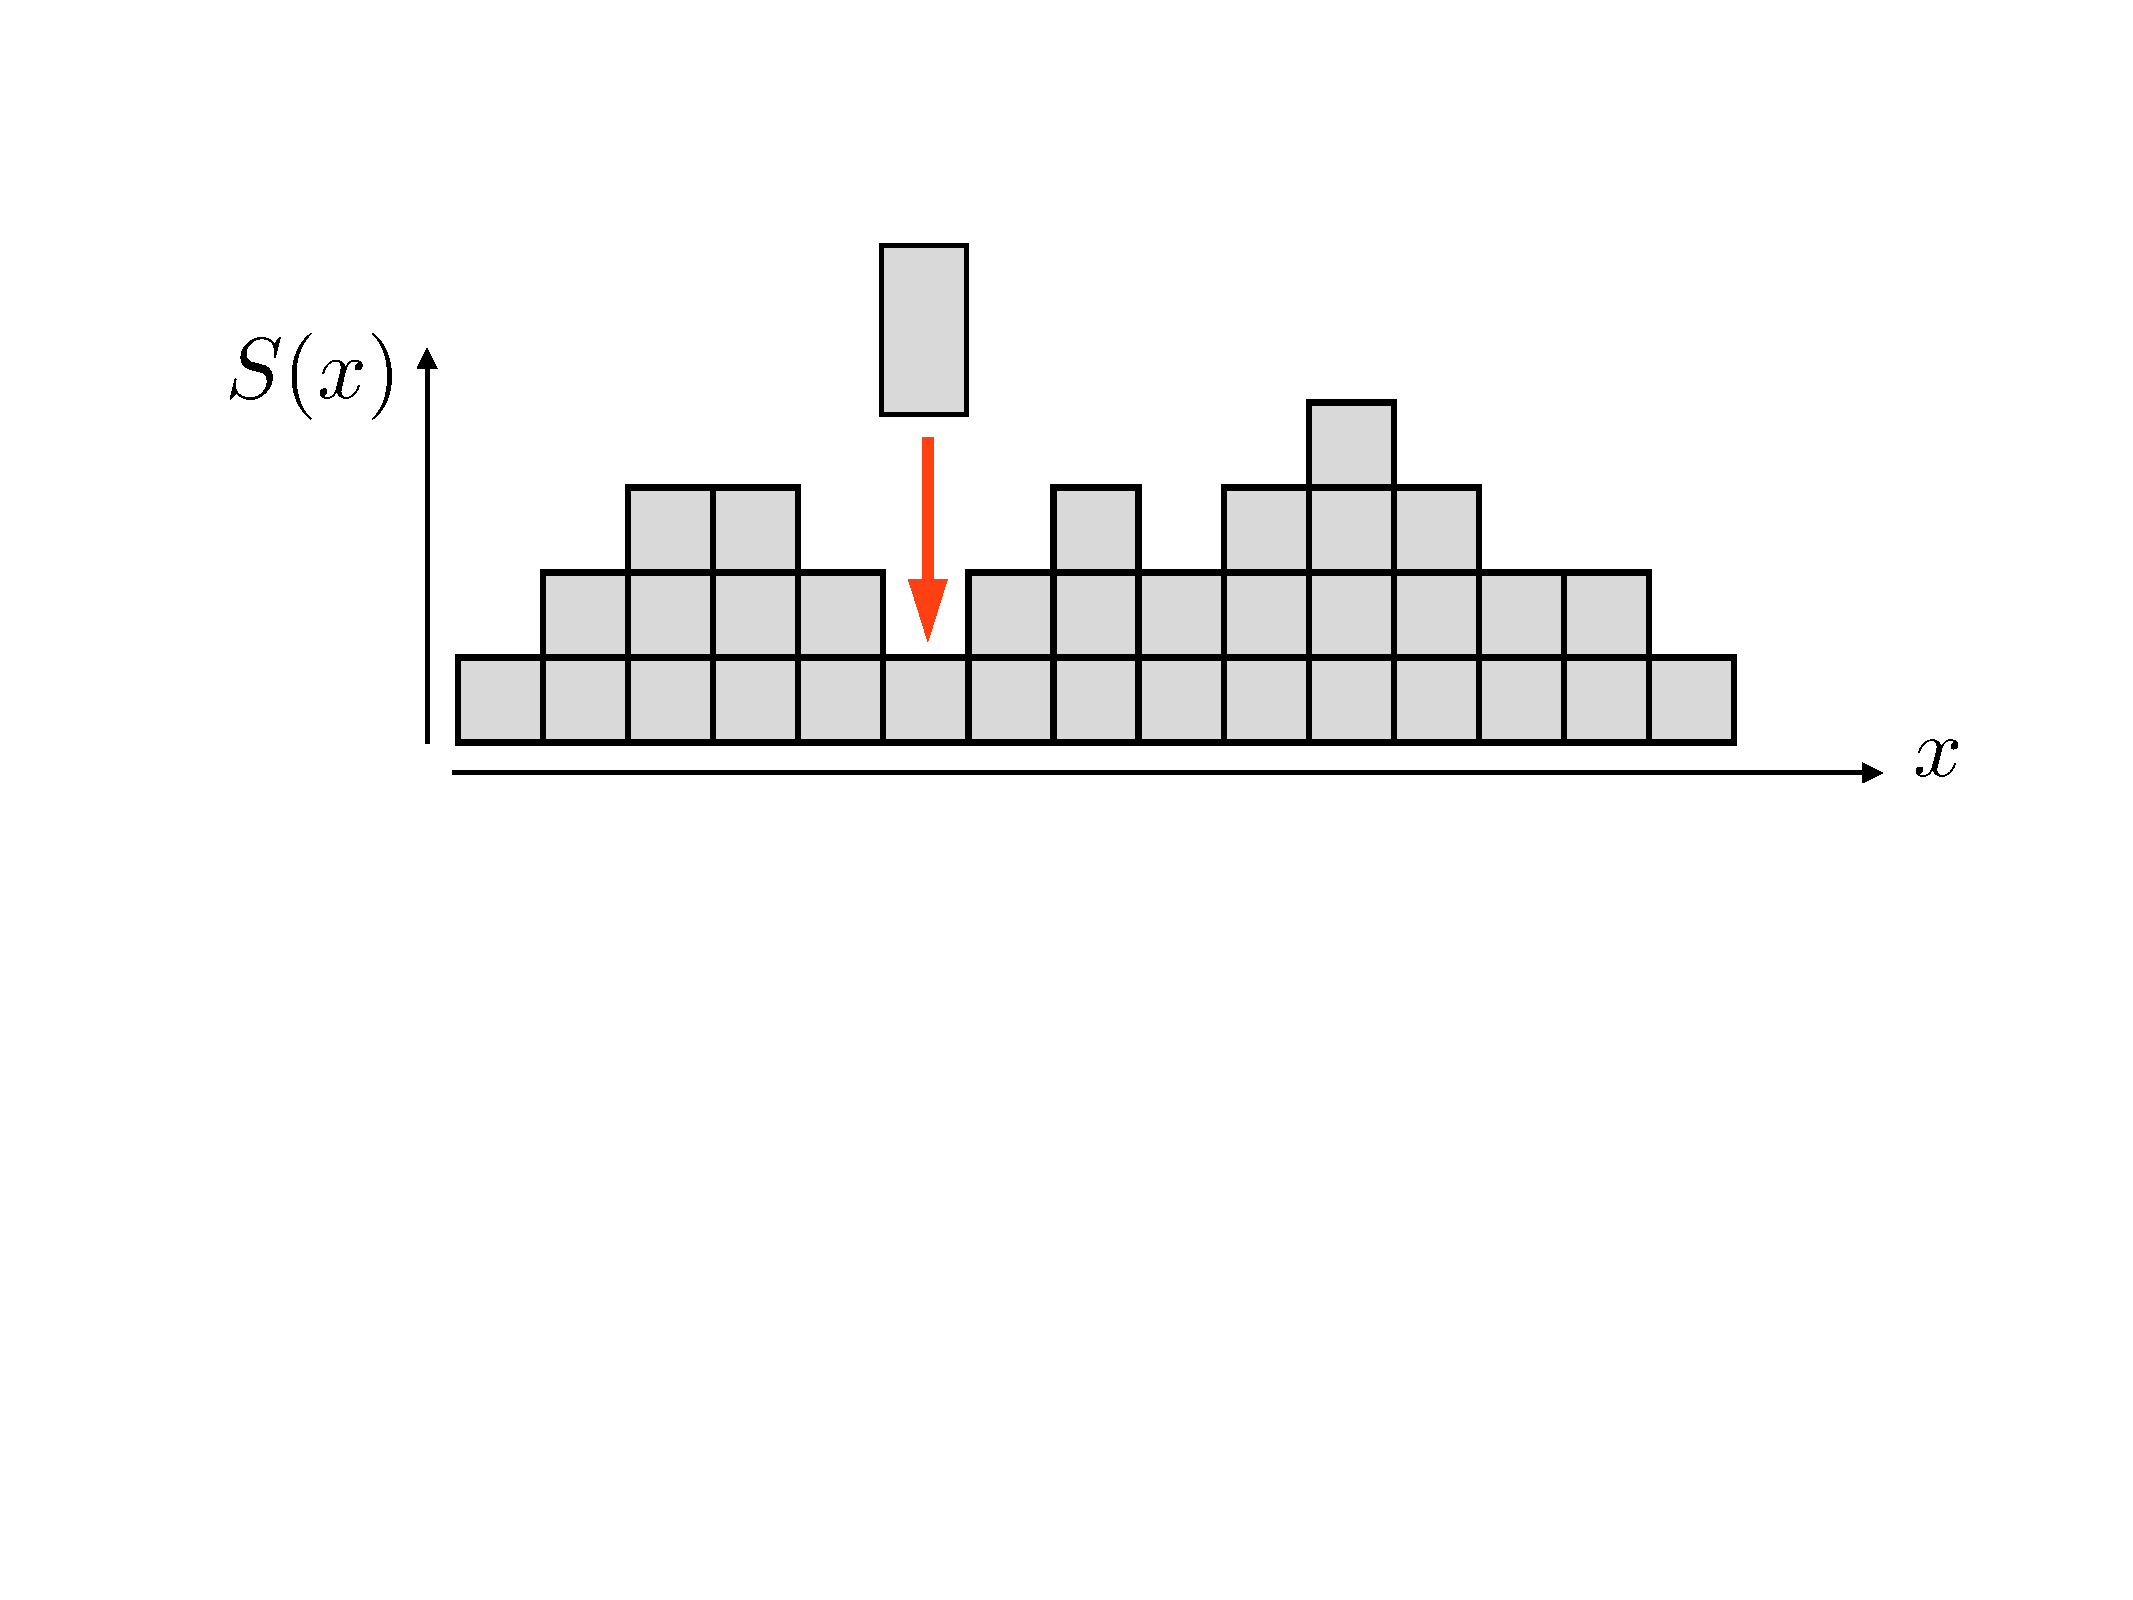
\includegraphics[width=.5\textwidth]{tetris.pdf}
	\caption{\textbf{Tetris-like model for large-$q$ chain.} The gate at cut $x$ adds enough entropy so that $S(x)$ is one greater than either of its neighbors. Figure from~\cite{Nahum2017}.}
	\label{fig:tetris}
\end{figure}
In general, it is possible for the entropy across two adjacent cuts to be equal. However, Fig.~\ref{fig:applyingUnitary}, also from~\cite{Nahum2017}, shows that flat sections can be destroyed but not created. 
\begin{figure}
	\centering
	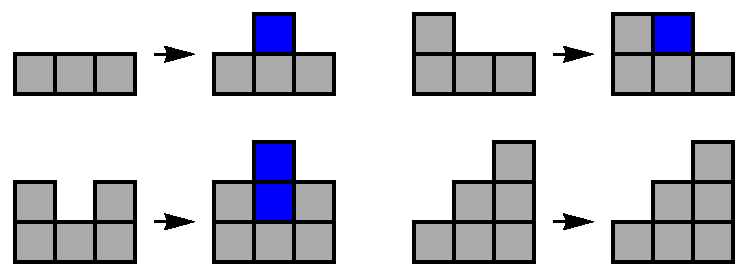
\includegraphics[width=.5\textwidth]{applyingUnitary.pdf}
	\caption{\textbf{Several possibilities for local changes} in the large $q$ model. If three adjacent cuts all have equal entropy, the two flat sections annihilate each other. There is no way to generate flat sections. Figure from~\cite{Nahum2017}.}
	\label{fig:applyingUnitary}
\end{figure}

If the system has been evolving for a long time, then, it makes sense then to only consider states that have no flat sections, so that $S(x) = S(x-1)\pm1$ for all $x$. In this case, instead of a picture like Fig.~\ref{fig:tetris} it is possible to represent the entropy at each bond as a point, with a diagonal slope connecting bonds. The slope between cuts (at a site) will always be $\pm1$. Instead of $2\times1$ or $1\times1$ rectangles, the gates are then squares coming down point-first, as in Fig.~\ref{fig:diaggate}. 
\begin{figure}
	\centering
	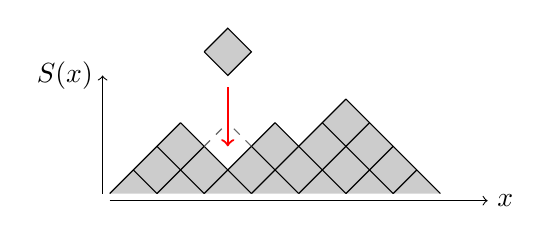
\begin{tikzpicture}[scale = .3]
\draw[->] (0, -.3) -- (16,-.3) node[right]{$x$};
\draw[->] (-.3,0) -- (-.3,5) node[left]{$S(x)$};
\fill[black!20] (0,0) -- (3,3) -- (5,1) -- (7,3) -- (8,2) --
				(10,4) -- (14,0) ;
\draw (0,0) -- (3,3);
\draw (2,0) -- (4,2);
\draw (4,0) -- (7,3);
\draw (6,0) -- (10,4);
\draw (8,0) -- (11,3);
\draw (10,0) -- (12,2);
\draw (12,0) -- (13,1);
\draw (2,0) -- (1,1);
\draw (4,0) -- (2,2);
\draw (6,0) -- (3,3);
\draw (8,0) -- (6,2);
\draw (10,0) -- (7,3);
\draw (12,0) -- (9,3);
\draw (14,0) -- (10,4);
\draw[dashed, black!60]  (4,2) -- (5,3);
\draw[dashed, black!60]  (6,2) -- (5,3);

\draw[fill=black!20] (4,6) -- (5,5) -- (6,6) -- (5,7) -- (4,6);
\draw[thick, ->, red] (5,4.5) -- (5,2);
\end{tikzpicture}
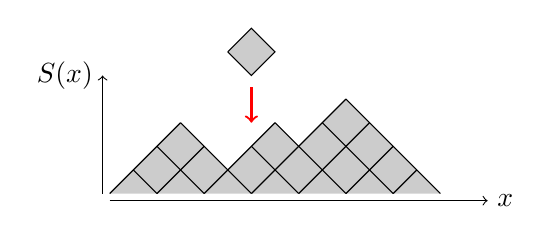
\begin{tikzpicture}[scale = .3, cross/.style={path picture={ 
		\draw[black]
		(path picture bounding box.south east) -- (path picture bounding box.north west) (path picture bounding box.south west) -- (path picture bounding box.north east);
}}]

\draw[->] (0, -.3) -- (16,-.3) node[right]{$x$};
\draw[->] (-.3,0) -- (-.3,5) node[left]{$S(x)$};
\fill[black!20] (0,0) -- (3,3) -- (5,1) -- (7,3) -- (8,2) --
(10,4) -- (14,0) ;
\draw (0,0) -- (3,3);
\draw (2,0) -- (4,2);
\draw (4,0) -- (7,3);
\draw (6,0) -- (10,4);
\draw (8,0) -- (11,3);
\draw (10,0) -- (12,2);
\draw (12,0) -- (13,1);
\draw (2,0) -- (1,1);
\draw (4,0) -- (2,2);
\draw (6,0) -- (3,3);
\draw (8,0) -- (6,2);
\draw (10,0) -- (7,3);
\draw (12,0) -- (9,3);
\draw (14,0) -- (10,4);
%\draw[dashed, black!60]  (5,3) -- (6,4);
%\draw[dashed, black!60]  (7,3) -- (6,4);
%\draw[dashed, black!60]  (6,2) -- (5,3);

\draw[fill=black!20] (5,6) -- (6,5) -- (7,6) -- (6,7) -- (5,6);
\draw[thick, ->, red] (6,4.5) -- (6,3);
%\node [draw,circle,cross,minimum width=1](B) at (6,3.5){}; 
\end{tikzpicture}

	\caption{\textbf{Another picture of the configuration in Fig.~\ref{fig:tetris}}. Here the cut positions are top or bottom vertices of the squares. On the left, the gate at time $t$ results in entropy growth at $x$ because at time $t-1$, $S(x-1) > S(x) < S(x+1)$. On the right the gate has no effect. Although $S(x) < S(x+1)$, the case $S(x) < S(x-1)$ is not satisfied. The bottom row of the picture is not made of squares because the state has been evolving for a long time.}
	\label{fig:diaggate}
\end{figure}
If the gate falls on a local minimum, it lifts the entropy at that bond. If the gate falls on a local maximum or a non-extremum it has no effect.

In this picture, we can describe an entropy curve as a series of up and down steps, with each step defined at a site (between two cuts), For example, the initial state in Fig.~\ref{fig:diaggate} would be $uuudduuduudddd$ and the final state would be $uuudududuudddd$. To make this look like a classical spin system (as in the Ising model), we can a state $s$, where $s_i$ is the local slope at site $i$, with $u\to1$ and $d\to-1$. This encoding provides simple expressions for the coarse-grained slope and correlation, which we will use in Sec.~\ref{sub:coarse}.

\subsubsection{Minimal Cut Picture} \label{subsub:mincut}

Using the fact that a productive gate raises the entropy at a cut by 2, we can use another picture of the dynamics based on Fig.~\ref{fig:brickcircuit}. Assume the initial state is a product state so the entropy at each cut is initially 0 and evolve with a brickwork circuit. Then after one of the first gates (for example between $i=3$ and $i=4$) the entropy at that cut will become 1. After any of the subsequent gates the entropy at the affected cut increases by 2.

The minimal cut picture~\cite{Nahum2017} reproduces this behavior by considering cuts through the circuit, as in Fig.~\ref{fig:mincut}.
\begin{figure}
	\centering
	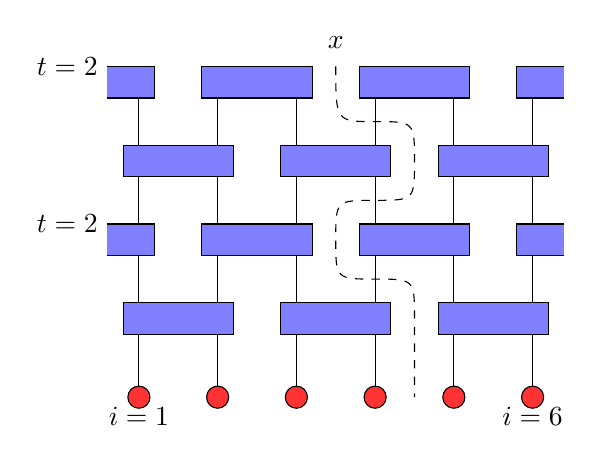
\begin{tikzpicture}[scale = 1]
\draw (0,0) node[below]{$i=1$} -- (0,4);
\filldraw[color=black, fill=red!80] (0,0) circle (4pt) node[anchor=west] { };
\draw (1,0) -- (1,4);
\filldraw[color=black, fill=red!80] (1,0) circle (4pt) node[anchor=west] { };
\draw (2,0) -- (2,4);
\filldraw[color=black, fill=red!80] (2,0) circle (4pt) node[anchor=west] { };
\draw (3,0) -- (3,4);
\filldraw[color=black, fill=red!80] (3,0) circle (4pt) node[anchor=west] { };
\draw (4,0) -- (4,4);
\filldraw[color=black, fill=red!80] (4,0) circle (4pt) node[anchor=west] { };
\draw (5,0) node[below]{$i=6$} -- (5,4);
\filldraw[color=black, fill=red!80] (5,0) circle (4pt) node[anchor=west] { };

\foreach \x/\y in {0/1, 2/1, 4/1, 1/2, 3/2, 0/3, 2/3, 4/3, 1/4, 3/4} 
\filldraw[color=black, fill=blue!50] (\x-.2,\y-.2) rectangle (\x+1.2,\y+.2);

\draw[fill=blue!50] (-.4,1.8) -- (.2,1.8) -- (.2,2.2) -- (-.4,2.2)
								node[left] {$t=2$};
\draw[fill=blue!50] (-.4,3.8) -- (.2,3.8) -- (.2,4.2) -- (-.4,4.2)
								node[left] {$t=2$};
\draw[fill=blue!50] (5.4,4.2) -- (4.8,4.2) -- (4.8,3.8) -- (5.4,3.8);
\draw[fill=blue!50] (5.4,2.2) -- (4.8,2.2) -- (4.8,1.8) -- (5.4,1.8);

\draw (2.5,4.5) node{$x$};
\draw[dashed] (2.5,4.2) .. controls (2.5,3.5) .. (3,3.5) 
                        .. controls (3.5,3.5) .. (3.5,3) 
                        .. controls (3.5,2.5) .. (3,2.5) 
                        .. controls (2.5,2.5) .. (2.5,2) 
                        .. controls (2.5,1.5) .. (3,1.5) 
                        .. controls (3.5,1.5) .. (3.5,1) 
                        .. controls (3.5,0.5) .. (3.5,0.5) 
                        .. controls (3.5,0.0) .. (3.5,0);
\end{tikzpicture}
	\caption{\textbf{Minimal cut picture.} Assuming an initial product state, $S(x)$ is given by the minimal number of legs that must be cut to draw a line from the bottom of the circuit to $x$. Cutting through gates is not allowed (or equivalently costs two cuts) and the initial point need not be $x$. Figure adapted from~\cite{Nahum2017}.}
	\label{fig:mincut}
\end{figure}
To find the entanglement across $x$, start in an unentangled state. If the initial state is entangled, include gates for $t<0$ that evolve a product state into the initial state at time $t=0$. Then, starting at the top of the circuit at $x$, find the path through the circuit that cuts through no gates and through the fewest of the lines defined by sites, called legs. The path need not end at $x$. The entanglement at $x$ is the number of legs cut by this path. 

For the brickwork circuit, this reproduces the entropy calculation quoted above, with first gates generating 1 unit of entanglement and subsequent gates generating 2. However, in circuits where not every gate is productive, the min-cut picture still works, and agrees with the surface growth picture.

Consider the circuit in Fig.~\ref{fig:degeneratemincut}.
\begin{figure}
	\centering
	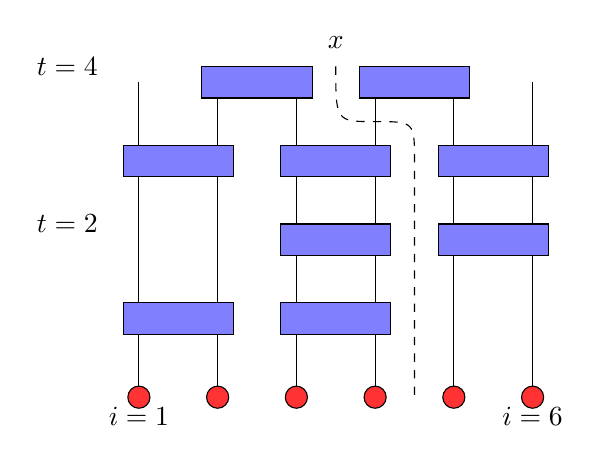
\begin{tikzpicture}[scale = 1]
\draw (0,0) node[below]{$i=1$} -- (0,4);
\filldraw[color=black, fill=red!80] (0,0) circle (4pt) node[anchor=west] { };
\draw (1,0) -- (1,4);
\filldraw[color=black, fill=red!80] (1,0) circle (4pt) node[anchor=west] { };
\draw (2,0) -- (2,4);
\filldraw[color=black, fill=red!80] (2,0) circle (4pt) node[anchor=west] { };
\draw (3,0) -- (3,4);
\filldraw[color=black, fill=red!80] (3,0) circle (4pt) node[anchor=west] { };
\draw (4,0) -- (4,4);
\filldraw[color=black, fill=red!80] (4,0) circle (4pt) node[anchor=west] { };
\draw (5,0) node[below]{$i=6$} -- (5,4);
\filldraw[color=black, fill=red!80] (5,0) circle (4pt) node[anchor=west] { };

\foreach \x/\y in {0/1, 0/3, 2/1, 2/2, 2/3, 4/2, 4/3, 1/4, 3/4} 
\filldraw[color=black, fill=blue!50] (\x-.2,\y-.2) rectangle (\x+1.2,\y+.2);

\draw[fill=blue!50] (-.4,2.2) node[left] {$t=2$};
\draw[fill=blue!50] (-.4,4.2) node[left] {$t=4$};

\draw (2.5,4.5) node{$x$};
\draw [dashed] (2.5,4.2) .. controls (2.5,3.5) .. (3,3.5) 
                         .. controls (3.5,3.5) .. (3.5,3) 
                         .. controls (3.5,1.5) .. (3.5,1) 
                         .. controls (3.5,0.5) .. (3.5,0.5) 
                         .. controls (3.5,0.0) .. (3.5,0);
\end{tikzpicture}
	\caption{\textbf{Minimal cut with degenerate gates.} All gates at cut $x$ after the first gate there produce no entanglement because $S(x)$ is a local maximum.}
	\label{fig:degeneratemincut}
\end{figure}
After the initial gate acts between sites 3 and 4, $S(x)$ becomes a local maximum, with so that all gates after it become unproductive. In the surface growth picture this is represented by multiple gates falling on a local maximum. This is to show that the min-cut picture agrees with the surface growth picture, and provides another set of intuition for the dynamics of this class of circuits.

Since cuts through gates can considered as having cost 2, there is one more equivalent picture for the min-cut procedure: at the location of each gate, cross, or ``tangle," the two relevant strands. Fig.~\ref{fig:anothermincut} shows this picture for the same circuit as in Fig.~\ref{fig:degeneratemincut}.
\begin{figure}
	\centering
	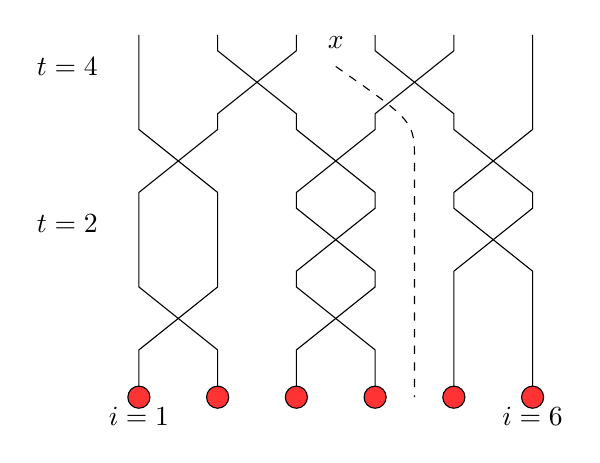
\begin{tikzpicture}[scale = 1]
\draw (0,0) node[below]{$i=1$} -- (0,.6) -- (1,1.4) -- (1,2.6) -- (0,3.4) -- (0,4.6);
\filldraw[color=black, fill=red!80] (0,0) circle (4pt) node[anchor=west] { };
\draw (1,0) -- (1,.6) -- (0,1.4) -- (0,2.6) -- (1,3.4) -- (1,3.6) -- (2,4.4) -- (2,4.6);
\filldraw[color=black, fill=red!80] (1,0) circle (4pt) node[anchor=west] { };
\draw (2,0) -- (2,.6) -- (3,1.4) -- (3,1.6) -- (2,2.4) -- (2,2.6) -- (3,3.4) -- (3,3.6) -- (4,4.4) -- (4,4.6);
\filldraw[color=black, fill=red!80] (2,0) circle (4pt) node[anchor=west] { };
\draw (3,0) -- (3,.6) -- (2,1.4) -- (2,1.6) -- (3,2.4) -- (3,2.6) -- (2,3.4) -- (2,3.6) -- (1,4.4) -- (1,4.6);
\filldraw[color=black, fill=red!80] (3,0) circle (4pt) node[anchor=west] { };
\draw (4,0) -- (4,1.6) -- (5,2.4) -- (5,2.6) -- (4,3.4) -- (4,3.6) -- (3,4.4) -- (3,4.6);
\filldraw[color=black, fill=red!80] (4,0) circle (4pt) node[anchor=west] { };
\draw (5,0) node[below]{$i=6$} -- (5,1.6) -- (4,2.4) -- (4,2.6) -- (5,3.4) -- (5,4.6);
\filldraw[color=black, fill=red!80] (5,0) circle (4pt) node[anchor=west] { };



\draw[fill=blue!50] (-.4,2.2) node[left] {$t=2$};
\draw[fill=blue!50] (-.4,4.2) node[left] {$t=4$};

\draw (2.5,4.5) node{$x$};
\draw [dashed] (2.5,4.2) .. controls (3.5,3.5) .. (3.5,3) 
                         .. controls (3.5,1.5) .. (3.5,1) 
                         .. controls (3.5,0.5) .. (3.5,0.5) 
                         .. controls (3.5,0.0) .. (3.5,0);
\end{tikzpicture}
	\caption{Another representation of the min-cut picture, with gates replaced by tangled strands. The advantage of this view is that gates clearly look like objects whose crossing has twice the cost of crossing a strand.}
	\label{fig:anothermincut}
\end{figure}

Instead of asking about the entanglement from $x$ to the bottom of the circuit, we can find the entanglement between $x$ and a specific bond position $y$ at the bottom of the circuit, where $x$ and $y$ are separated by time $t$. This is the entanglement of the time evolution operator $U(t)$, and will be denoted $S_U(y,x,t)$~\cite{Jonay18}. Then the entanglement is just the cost of the minimal cut from $x$ to $y$. There are two reasons this is a useful quantity. Once is in finding the entanglement of operators, as the space of operators behaves like a doubled space of state~\cite{Jonay17, Jonay18}. Alternatively, if we want to find $S(x)$ for an arbitrary initial entanglement, we can compute $S(x,y)$, and then $S(x) = \min_y\{S(x,y) + S_0(y)\}$.

\subsection{Coarse Graining and Long Wavelength Dynamics} \label{sub:coarse}

It is possible to abstract out even more of the detailed dynamics to consider the large scale behavior. To do this, interpret $S(x)$ as a continuous real valued function. The entanglement growth rate can be calculated under the assumption that up and down steps (from the picture in Fig.~\ref{fig:diaggate}) are uncorrelated and the large scale slope $\pd{S}{x}$ is constant. These assumptions hold only in the stead state of the random (1-stair) architecture. However, they are a useful first-order approximation to the behavior of other length stair circuits.

For an entropy surface with constant slope $m\equiv\pd{S}{x}$ and no correlations, each step from one site to the next has probability $\frac{1+m}{2}$ of being up and $\frac{1-m}{2}$ of being down. The assumption that there are no correlations is exact in the random architecture. Consider a gate operating on cut $x$ at time $t$. For the gate to increase the entropy $S(x)$, it must be the case that $S(x)<S(x-1), S(x+1)$. The probability of this is $\frac{1+m}{2} \frac{1-m}{2} = \frac{1-m^2}{4}$. In this case we have $S(x,t+1)=S(x,t)+2$, because the gate increases the entropy to be great than that of its neighbors. Then if the gates arrive at each cut with a rate $\gamma$, the entanglement growth rate is
\begin{align}
\pd{S}{t} = \gamma\frac{1-m^2}{2}\equiv \Gamma(m). \label{eqn:randomgrowthrate}
\end{align}
Useful checks of this formula are that the entropy does not increase at maximal or minimal slope $m=1,-1$, and that at $m=0$, $\pd{S}{t}=\gamma/2$, 1/4 the brickwork value, since $1/4$ of the gates are productive. The latter rate makes sense because in the case of the brickwork circuit all gates are guaranteed to raise the entropy, while here only 1/4 will have an effect.

\subsubsection{Entanglement Velocity} \label{subsub:v_E }

$\Gamma(m)$ contains encodes a significant amount of information about the entanglement growth of the system~\cite{Jonay18}, and is useful in calculating both the entanglement velocity and the butterfly velocity. We will discuss this function in more detail and show how these speeds can be extracted.

Consider a linear section of the entanglement curve $S(x,t)$, and its evolution through time $\tau$. We know that $S(y,t+\tau) = \min_x\{S_U(y,x,\tau) + S(x,t)\}$. If we assume the gate architecture is translationally invariant (which is true in the large-scale limit) then $S_U(y,x,\tau)$ depends only on the slope $v = \frac{y-x}{\tau}$, multiplied by the length of the cut from $x$ to $y$. Graphically, this corresponds to Fig.~\ref{fig:legendre}.
\begin{figure}
	\centering
	\begin{tikzpicture}
\draw (0,0) node[left]{$t+\tau$} -- (8,0);
\draw (0,3) node[left]{$t$}      -- (8,3);
\draw (4,0) -- (7,3);
\draw (4,-.1) node[below]{$x = y-vt$} -- (4,.1);
\draw (7,2.9) -- (7,3.1) node[above]{$y$};
\draw (1,-.1) node[below]{$x = 0$} -- (1,.1);
\draw (7,-.1) node[below]{$x = y$} -- (7,.1);
\end{tikzpicture}
	\caption{\textbf{Graphical interpretation of the Legendre transform.} Since the architecture is spacially homogeneous, $S_U$ depends only on the length and slope of the cut and is $S_U(y,x,\tau) \equiv G(v)\tau$, where $v=(x-y)/\tau$.}
	\label{fig:legendre}
\end{figure}
Since we assumed the initial state was linear, we can write it as $S(x,t) = mx = mv\tau+my$. From the linearity of $S_U$, and the fact that its only other dependence is on $v$, we can define $S_U(y,x,\tau) \equiv G(v)\tau$. 

The final entanglement $S(y,t+\tau) = \min_x\{G(v)\tau + mv\tau\}$ can be differentiated with respect to $\tau$ to obtain.
\begin{align}
\Gamma(m) = \min_v\{G(v) + mv\}.
\end{align}
Ref.~\cite{Jonay18} contains this equation with an extra factor of $m_\text{eq}$, the equilibrium slope. In the large-$q$ random circuits we are considering, this slope is 1 due to the saturation of Eq.~\ref{eqn:offbyone}.

One useful fact about $\Gamma(m)$ is that it is convex. If it were not, then there would be some $m^*$ such that $\Gamma(m^*+\eps), \Gamma(m^*-\eps)<\Gamma(m^*)$. However, if this is the case, we can always draw a jagged path from $x$ to $y$ alternating between slopes $m^*+\eps$ and $m^*-\eps$. This path with have average slope $m$ but have a higher growth rate than $\Gamma(m)$. Therefore we have reached a contradiction and $\Gamma(m)$ is convex.

We can use the coarse-grained dynamics to reproduce the calculation of the entanglement velocity in Eq.~\ref{eqn:vE}. The entanglement velocity is the speed at which the kinks between the flat section $m=0$ and the sloped sections $m=\pm1$ move in the coarse grained version of Fig.~\ref{fig:Tower}. The sloped section does not move up, while the flat section moves up at $\Gamma(0)$. To preserve the continuity of $S(x)$, the kinks have to move at $v_E=\Gamma(0)$. Fig.~\ref{fig:entanglevel} shows this calculation of $v_E$.
\begin{figure}
	\centering
	\begin{tikzpicture}
\draw[->] (-.5,0) -- (5,0) node[below right]{$x$};
\draw[->] (0,-.5) -- (0,4) node[below left]{$S(x,t)$};
\draw[] (0,1) -- (3.5,1) -- (4.5,0);
\draw[->] (1,1.3) -- (1,2.2) ;
\draw (1.5,1.5) node{\small $\Gamma(0)$};
\draw (0,2.5) -- (2,2.5) -- (3.5,2.5);
\draw[dashed] (2,2.5) -- (3.5,1);
\draw[->] (3.2,3) -- (2,3) node[above right]{\small $v_E$};
\draw (4.5,.8) node{\small $m=-1$};
\draw (1.5,.7) node{\small $m=0$};
\end{tikzpicture}
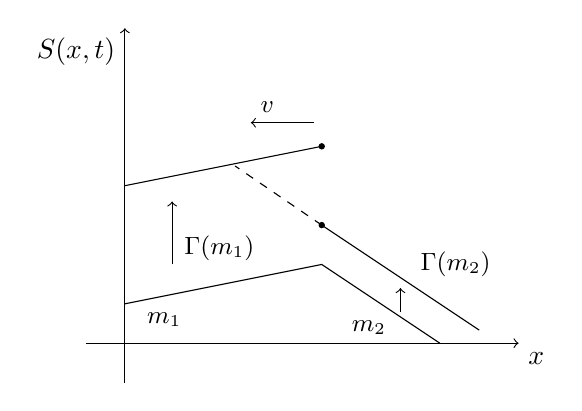
\begin{tikzpicture}
\draw[->] (-.5,0) -- (5,0) node[below right]{$x$};
\draw[->] (0,-.5) -- (0,4) node[below left]{$S(x,t)$};
\draw (0,0.5) -- (2.5,1) -- (4,0);
\draw (0,2) -- (2.5,2.5) node[draw,shape=circle, fill=black, scale=.2]{} (2.5,1.5) node[draw,shape=circle, fill=black, scale=.2]{} -- (4,.5) -- (4.5,.1666);
\draw[->] (.6,1) -- (.6,1.8) ;
\draw[->] (3.5,.4) -- (3.5,.7) ;
\draw (1.2,1.2) node{\small $\Gamma(m_1)$}
      (0.5,0.3) node{\small $m_1$}
      (4.2,1.0) node{\small $\Gamma(m_2)$}
      (3.1,0.2) node{\small $m_2$};
\draw[dashed] (2.5,1.5) -- (1.4,2.25);
\draw[->] (2.4,2.8) -- (1.6,2.8) node[above right]{\small $v$};
\end{tikzpicture}
	\caption{\textbf{Entanglement velocity in the surface growth picture.} The left figure shows a flat slope rising at $\Gamma(0)$. The $m=-1$ section does not grow. The flat slope would rise to the shown line, but the right end is held down by the entanglement bounds. The dashed line shows the corrected $S(x)$. On the right both sections grow at the growth rates defined by their slopes. To maintain continuity the kink moves at $v=-\frac{\Gamma(m_2)-\Gamma(m_1)}{m_2-m_1}$.}
	\label{fig:entanglevel}
\end{figure}

The same figure can be used to calculate the velocity of a kink between arbitrary slopes, as long as the kink is a local maximum. In this case the vertical distance between the two solid line endpoints is $(\Gamma(m_1)-\Gamma(m_2))t$. This must be equal to the total vertical rise along the two slopes, $(m_1-m_2)\left(\frac{-v}{t}\right)$, where $\frac{-v}{t}$ is the horizontal distance between the initial and final positions of the feature. Altogether, $v=-\frac{\Gamma(m_2)-\Gamma(m_1)}{m_2-m_1}$. For $m_1=0, m_2=-1$ this reduces to $v_E=\Gamma(0)$.

This expression has a nice interpretation in terms of the growth rate $\Gamma(m)$. It is the slope a chord drawn on the growth rate function between points corresponding to the two slopes, as in Fig.~\ref{fig:growthchord}.
\begin{figure}
	\centering
	\begin{tikzpicture}
\draw[->] (-3,0) -- (3,0) node[below right]{$m$};
\draw[->] (0,-.5) -- (0,3) node[below left]{$\Gamma(m)$};
\draw[domain=-2:2] plot (\x, {2-\x*\x/2});
\draw (-2,-.1) node[below]{\footnotesize $m=-1$} -- (-2,.1);
\draw (-2,0) -- (0,2);
\end{tikzpicture}
\quad
\begin{tikzpicture}
\draw[->] (-3,0) -- (3,0) node[below right]{$m$};
\draw[->] (0,-.5) -- (0,3) node[below left]{$\Gamma(m)$};
\draw[domain=-2:2] plot (\x, {2-\x*\x/2});
\draw (.4,-.1) node[below]{\footnotesize $m_1$} -- (.4,.1);
\draw (-.75,-.1) node[below]{\footnotesize $m_2$} -- (-.75,.1);
\draw (.4, 2-.4*.2) -- (-.75, 2-.75*.75/2);
\end{tikzpicture}
	\caption{\textbf{Calculation of kink speed from chord,} using the growth rate for random circuits, Eq.~\ref{eqn:randomgrowthrate}.Note that the chord slopes are positive, while the corresponding velocities (Fig.~\ref{fig:entanglevel}) are negative.}
	\label{fig:growthchord}
\end{figure}

\subsubsection{Butterfly Velocity} \label{subsub:v_B}

The same calculation does not work if the kink is a local minimum, as these features do not remain sharp. This is because a perturbation to the kink will travel up faster than either side of the kink, filling in the kink with a smooth curve. There is a well defined point where this curve hits the linear section with slope $m$ at a tangent. It is possible to calculate the speed at which this point moves (see Fig.~\ref{fig:buttvel}).
\begin{figure}
	\centering
	\begin{tikzpicture}
\draw[->] (-.5,0) -- (5.5,0) node[below right]{$x$};
\draw[->] (0,-.5) -- (0,5) node[below left]{$S(x,t)$};
\draw (0,3) -- (3,.5) node[draw,shape=circle, fill=black, scale=.2]{} -- (5,2);
\draw (0,3.5) -- (2,1.833) node[draw,shape=circle, fill=black, scale=.2]{}
	.. controls (51/19,1.263) ..
	(3.5,1.875) node[draw,shape=circle, fill=black, scale=.2]{} -- (5,3);
\draw[dashed] (2,1.833) -- (51/19,1.263) -- (3.5,1.875);
\draw (1.4,1.3) node{\footnotesize $m_1$};
\draw (4.2,1) node{\footnotesize $m_2$};
\end{tikzpicture}
\begin{tikzpicture}
\draw[->] (-.5,0) -- (5.5,0) node[below right]{$x$};
\draw[->] (0,-.5) -- (0,4) node[below left]{$S(x,t)$};
\draw (0,3) --(2.5,.5) node[draw,shape=circle, fill=black, scale=.2]{} -- (5,3);
\draw (0,3) -- (1.5,1.5) node[draw,shape=circle, fill=black, scale=.2]{}
	.. controls (2.5,.5) ..
	(3.5,1.5) node[draw,shape=circle, fill=black, scale=.2]{} -- (5,3);
%\draw[dashed] (1.5,1.5) -- (2.5,.5) -- (3.5,1.5);
\draw (1,1) node{\footnotesize $m_1=1$};
\draw (4,1) node{\footnotesize $m_2=-1$};
\end{tikzpicture}
	\caption{\textbf{Velocity of tangent points.} On the left, the left and right points move at $v=-\Gamma'(m_1)$ and $v=-\Gamma'(m_2)$ respectively. On the right these two speeds are the butterfly speeds, $-\Gamma'(\pm1) = \mp v_B$. Since both slopes are extremal, the linear sections do not grow.}
	\label{fig:buttvel}
\end{figure}
Since this tangent point is the limiting case of a cusp where the two slopes $m_1$ and $m_2$ approach each other. This turns the calculation of the chord slope into a calculation of the tangent to the entanglement growth curve at $m$, $\Gamma'(m)$. Since $\Gamma(m)$ is convex, this is the largest slope attainable by a chord or tangent line, so $v_B$ is the fastest possible speed for a feature on the entanglement function.

Although it is not obvious, the butterfly is given by the speed of tangent points on maximal slope sections, $v_B = -\Gamma'(m_{\text{max}})$. This connection holds in general, but is clearer in the random circuits considered here.

When the slope is near its largest possible value, so that the entropy increases at nearly every site, it is possible to isolate the behavior of the few down steps. Figure~\ref{fig:particle} shows such a configuration.
\begin{figure}
	\centering
	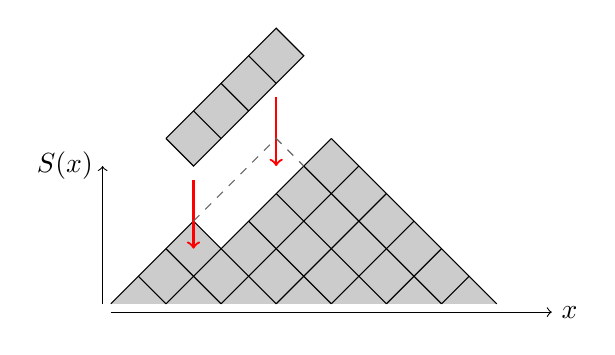
\begin{tikzpicture}[scale = .35]
\draw[->] (0, -.3) -- (16,-.3) node[right]{$x$};
\draw[->] (-.3,0) -- (-.3,5) node[left]{$S(x)$};
\fill[black!20] (0,0) -- (3,3) -- (4,2) -- (8,6) -- (14,0) ;
\draw (0,0) -- (3,3);
\draw (2,0) -- (8,6);
\draw (4,0) -- (9,5);
\draw (6,0) -- (10,4);
\draw (8,0) -- (11,3);
\draw (10,0) -- (12,2);
\draw (12,0) -- (13,1);
\draw (2,0) -- (1,1);
\draw (4,0) -- (2,2);
\draw (6,0) -- (3,3);
\draw (8,0) -- (5,3);
\draw (10,0) -- (6,4);
\draw (12,0) -- (7,5);
\draw (14,0) -- (8,6);

\draw[fill=black!20] (2,6) -- (3,5) -- (4,6) -- (5,7) -- (6,8) -- (7,9) --
					 (6,10) -- (3,7) -- (2,6);
\draw (4,6) -- (3,7);
\draw (5,7) -- (4,8);
\draw (6,8) -- (5,9);
%\draw (9,9) -- ()
\draw[thick, ->, red] (3,4.5) -- (3,2);
\draw[thick, ->, red] (6,7.5) -- (6,5);

\draw[dashed, black!60] (3,3) -- (6,6) -- (7,5);
\end{tikzpicture}
	\caption{\textbf{Near-maximal slope}. The single down step acts like a particle in the system. The 4 consecutive gates have the effect of moving the particle 3 sites to the right.}
	\label{fig:particle}
\end{figure}
Since gates can only act between a down step and an up step, these ``particles" follow a deterministic behavior for a given architecture and control the entropy growth in the circuit. 

Consider a series of consecutive gates with its first gate acting between sites $i$ and $i+1$ and its last gate between $j$ and $j+1$. Series of gates like this (called staircases) are discussed in Sec.~\ref{sec:stairs}. If there are no down steps in this region, the gate has no effect. If there is a single down step somewhere between sites $i$ and $j$, inclusive, that step gets moved to site $j+1$. More down steps will interact with each other but at the present we are only considering configurations with isolated down steps. 

Now consider an operator with the last non-identity contribution at a site between $i$ and $j$, inclusive. With probability 1, the series of gates in the last paragraph move the end of the operator to site $j+1$. This demonstrates that operator ends and down step ``particles" have the same dynamics. The speed of the end of the operator is $v_B$. Since the particle has the same dynamics as the operator end, it also moves at velocity $v_B$. 

All that remains is to show how the speed of the particle is connected to $\Gamma(m)$. If there are $N$ down steps in a section of length $L$, then the slope is $m = 1-\frac{2N}{L}$. Furthermore, in time $t$ each down slope moves $v_Bt$, so the entropy growth is $\Gamma(m)=\frac{2Nv_B}{L}$. Plugging in for $m$, this gives
\begin{align}
\Gamma(m) &= v_B\left(\frac{2N}{L}\right) = v_B(1-m),\\
\left.\pd{\Gamma}{m}\right|_{m=0}  &= -v_B.
\end{align}

The previous discussion assumed that the particles are far enough from each other that they do not interfere with each other's dynamics. This is valid in the large $m$ limit as long as the particles are not attracted to each other. They could only affect each other if they are closer than a single series of gates. Then the early gates move the first particle until it is touching the second. At this point there are 2 down steps in a row and the next gate has no effect. The following gate lands on a local minimum and is able to move the second down slope to the end of the series of gates.

An equivalent description of these dynamics is that when a series of gates falls over two particles, the first one moves to just behind the second one, and then the second one moves to the end of the series of gates. Therefore the second one moves the distance it would without the first, while the first moves less than it would have if the second had not gotten in its way. This means that the particles are uncorrelated when far apart, and repel when they get too close. Therefore the uncorrelated assumption is correct. 
%\section{Dynamics in Asymmetric Circuits} \label{sec:stairs}

\subsection{Staircase Models}\emph{} \label{sub:stairs}

An interesting generalization of the random architecture is to consider ``staircases," which each consist of a series of gates, acting at cuts $x$, $x+1$, $x+2$, in sequential order. This would be a staircase moving to the right, but they can also move to the left. If there are $n$ gates in a staircase it is called an $n$-stair. They are called staircases because compared to figure~\ref{fig:tetris} they look like steps, as in figure~\ref{fig:stairs}. 
\begin{figure}
	\centering
	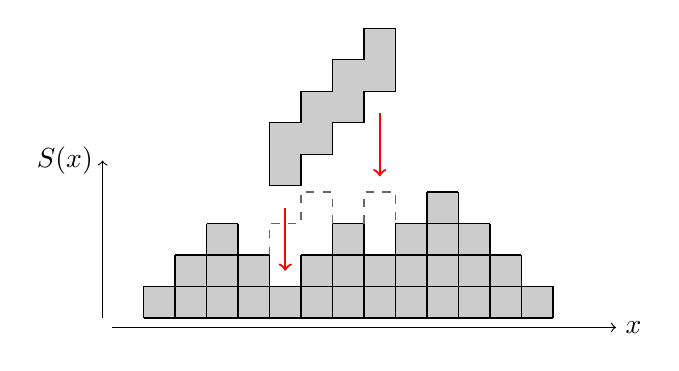
\begin{tikzpicture}[scale = .4]
\draw[->] (0, -.3) -- (16,-.3) node[right]{$x$};
\draw[->] (-.3,0) -- (-.3,5) node[left]{$S(x)$};
\fill[black!20] (1,0) -- (1,1) -- (2,1) -- (2,2) -- (3,2) -- (3,3) -- 
     			(4,3) -- (4,2) -- (5,2) -- (5,1) -- (6,1) -- (6,2) -- (7,2) -- (7,3) -- (8,3) -- (8,2) -- (9,2) -- (9,3) -- (10,3) -- (10,4) 
     			 -- (11,4) -- (11,3) -- (12,3) -- (12,2) -- (13,2) -- (13,1)  -- (14,1) -- (14,0);
     			 
\draw (1,0) -- (14,0);
\draw (1,1) -- (14,1);
\draw (2,2) -- (5,2);
\draw (6,2) -- (13,2);
\draw (3,3) -- (4,3);
\draw (7,3) -- (8,3);
\draw (9,3) -- (12,3);
\draw (10,4) -- (11,4);
\draw (1,0) -- (1,1);
\draw (2,0) -- (2,2);
\draw (3,0) -- (3,3);
\draw (4,0) -- (4,3);
\draw (5,0) -- (5,2);
\draw (6,0) -- (6,2);
\draw (7,0) -- (7,3);
\draw (8,0) -- (8,3);
\draw (9,0) -- (9,3);
\draw (10,0) -- (10,4);
\draw (11,0) -- (11,4);
\draw (12,0) -- (12,3);
\draw (13,0) -- (13,2);
\draw (14,0) -- (14,1);

\draw[fill=black!20] (5,5.2) -- (5,4.2) -- (6,4.2) -- (6,5.2) -- (7,5.2) --  
                     (7,6.2) --
					 (8,6.2) -- (8,7.2) -- (9,7.2) -- (9,8.2) -- (9,9.2) -- (8,9.2)
					 -- (8,8.2) -- (7,8.2) -- (7,7.2) -- (6,7.2) -- (6,6.2) -- (5,6.2)
					 -- (5,5.2);
\draw[thick, ->, red] (5.5,3.5) -- (5.5,1.5);
\draw[thick, ->, red] (8.5,6.5) -- (8.5,4.5);

\draw[dashed, black!60] (5,2) -- (5,3) -- (6,3) -- (6,4) -- (7,4) -- (7,3);
\draw[dashed, black!60] (8,3) -- (8,4) -- (9,4) -- (9,3);
\end{tikzpicture}
%\begin{tikzpicture}[scale = .3, cross/.style={path picture={ 
%		\draw[black]
%		(path picture bounding box.south east) -- (path picture bounding box.north west) (path picture bounding box.south west) -- (path picture bounding box.north east);
%}}]
%
%\draw[->] (0, -.3) -- (16,-.3) node[right]{$x$};
%\draw[->] (-.3,0) -- (-.3,5) node[left]{$S(x)$};
%\fill[black!20] (0,0) -- (3,3) -- (5,1) -- (7,3) -- (8,2) --
%(10,4) -- (14,0) ;
%\draw (0,0) -- (3,3);
%\draw (2,0) -- (4,2);
%\draw (4,0) -- (7,3);
%\draw (6,0) -- (10,4);
%\draw (8,0) -- (11,3);
%\draw (10,0) -- (12,2);
%\draw (12,0) -- (13,1);
%\draw (2,0) -- (1,1);
%\draw (4,0) -- (2,2);
%\draw (6,0) -- (3,3);
%\draw (8,0) -- (6,2);
%\draw (10,0) -- (7,3);
%\draw (12,0) -- (9,3);
%\draw (14,0) -- (10,4);
%\draw[dashed, black!60]  (5,3) -- (6,4);
%\draw[dashed, black!60]  (7,3) -- (6,4);
%\draw[dashed, black!60]  (6,2) -- (5,3);
%
%\draw[fill=black!20] (5,6) -- (6,5) -- (7,6) -- (6,7) -- (5,6);
%\draw[thick, ->, red] (6,4.5) -- (6,3);
%%\node [draw,circle,cross,minimum width=1](B) at (6,3.5){}; 
%\end{tikzpicture}

	\caption{\textbf{Staircase circuit architecture,} in which the gate at site $x$ is always followed by ones at sites $x+1, x+2$, making this a 3-stair. Note that not all gates are productive, only the ones that fall on sites that are local minima when they fall.}
	\label{fig:stairs}
\end{figure}
However, in the picture in which all sites are either up or down slopes, $n$-stair look like $n\times 1$ rectangles tilted $45^\circ$, as in figure~\ref{fig:diagstairs}.
\begin{figure}
	\centering
	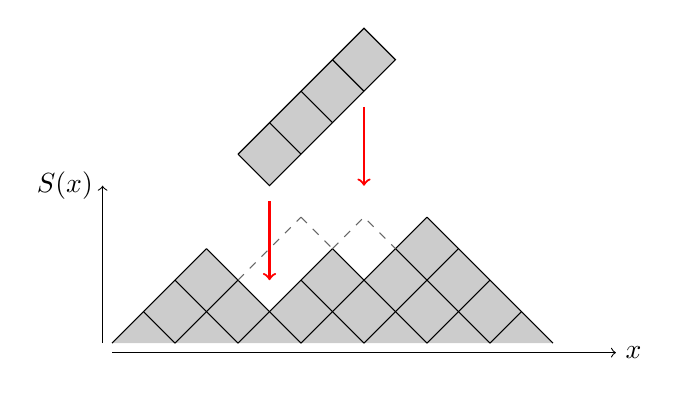
\begin{tikzpicture}[scale = .4]
\draw[->] (0, -.3) -- (16,-.3) node[right]{$x$};
\draw[->] (-.3,0) -- (-.3,5) node[left]{$S(x)$};
\fill[black!20] (0,0) -- (3,3) -- (5,1) -- (7,3) -- (8,2) --
				(10,4) -- (14,0) ;
\draw (0,0) -- (3,3);
\draw (2,0) -- (4,2);
\draw (4,0) -- (7,3);
\draw (6,0) -- (10,4);
\draw (8,0) -- (11,3);
\draw (10,0) -- (12,2);
\draw (12,0) -- (13,1);
\draw (2,0) -- (1,1);
\draw (4,0) -- (2,2);
\draw (6,0) -- (3,3);
\draw (8,0) -- (6,2);
\draw (10,0) -- (7,3);
\draw (12,0) -- (9,3);
\draw (14,0) -- (10,4);

\draw[fill=black!20] (4,6) -- (5,5) -- (6,6) -- (7,7) -- (8,8) -- (9,9) --
					 (8,10) -- (7,9) -- (6,8) -- (5,7) -- (4,6);
\draw (6,6) -- (5,7);
\draw (7,7) -- (6,8);
\draw (8,8) -- (7,9);
%\draw (9,9) -- ()
\draw[thick, ->, red] (5,4.5) -- (5,2);
\draw[thick, ->, red] (8,7.5) -- (8,5);

\draw[dashed, black!60] (4,2) -- (6,4);
\draw[dashed, black!60] (6,4) -- (7,3);
\draw[dashed, black!60] (7,3) -- (8,4) -- (9,3);
\end{tikzpicture}
%\begin{tikzpicture}[scale = .3, cross/.style={path picture={ 
%		\draw[black]
%		(path picture bounding box.south east) -- (path picture bounding box.north west) (path picture bounding box.south west) -- (path picture bounding box.north east);
%}}]
%
%\draw[->] (0, -.3) -- (16,-.3) node[right]{$x$};
%\draw[->] (-.3,0) -- (-.3,5) node[left]{$S(x)$};
%\fill[black!20] (0,0) -- (3,3) -- (5,1) -- (7,3) -- (8,2) --
%(10,4) -- (14,0) ;
%\draw (0,0) -- (3,3);
%\draw (2,0) -- (4,2);
%\draw (4,0) -- (7,3);
%\draw (6,0) -- (10,4);
%\draw (8,0) -- (11,3);
%\draw (10,0) -- (12,2);
%\draw (12,0) -- (13,1);
%\draw (2,0) -- (1,1);
%\draw (4,0) -- (2,2);
%\draw (6,0) -- (3,3);
%\draw (8,0) -- (6,2);
%\draw (10,0) -- (7,3);
%\draw (12,0) -- (9,3);
%\draw (14,0) -- (10,4);
%%\draw[dashed, black!60]  (5,3) -- (6,4);
%%\draw[dashed, black!60]  (7,3) -- (6,4);
%%\draw[dashed, black!60]  (6,2) -- (5,3);
%
%\draw[fill=black!20] (5,6) -- (6,5) -- (7,6) -- (6,7) -- (5,6);
%\draw[thick, ->, red] (6,4.5) -- (6,3);
%%\node [draw,circle,cross,minimum width=1](B) at (6,3.5){}; 
%\end{tikzpicture}

	\caption{\textbf{Another picture of the staircase architecture.} Note that this picture results in the same final state.}
	\label{fig:diagstairs}
\end{figure}

\subsection{Behavior Ignoring Correlations} \emph{}\label{sub:anal}

Under certain approximations the entanglement entropy behaves analytically. One important approximation (described in section \ref{subsub:determ}) is that the Hilbert space at each site is large enough that almost all gates will in general maximally entangle the two sites on which they act. Other simplifying assumptions include ignoring correlations in ups and downs and ignoring second- and higher-order derivatives in $S(x,t)$. Combining these two assumptions, we arrive at uncorrelated entropy environments, which may be described only by their slope, $m$.

\subsubsection{Small Stairs} \label{subsub:smallstairs} \emph{}

The smallest stairs are 1-stairs, which are just individual gates. For an entropy surface with constant slope $m$ and no correlations, each step from one site to the next has probability $\frac{1+m}{2}$ of being up and $\frac{1-m}{2}$ of being down. The assumption that there are no correlations is exact in the 1-stair case. Consider a gate operating on site $n$ at time $t$. For the gate to increase the entropy $S(n)$, it must be the case that $S(n)<S(n-1), S(n+1)$. The probability of this is $\frac{1+m}{2} \frac{1-m}{2} = \frac{1-m^2}{4}$. In this case we have $S(n,t+1)=S(n,t)+2$, because the gate increases the entropy to be great than that of its neighbors. Then if the gates arrive with a rate $\Gamma$, we have
\begin{align}
\pd{S}{t} = \Gamma\frac{1-m^2}{2}.
\end{align}
Useful checks of this formula are that the entropy does not increase at maximal or minimal slope $m=1,-1$, and that at $m=0$, $\pd{S}{t}=\Gamma/2$, half the brickwork value. The latter rate makes sense because in the case of the brickwork circuit all gates are guaranteed to raise the entropy, while here only half\footnote{Fix this} will have an effect.

2-stairs consist of one gate acting at site $n$ and one at site $n+1$. The entropy production of these gates is affected by the slope between them and the two slopes on either side. There are 8 possible configurations of those three slopes, but only 4 result in entropy growth, as shown in table~\ref{tab:2stair}. Although there will be correlation built up by the 2-stair architecture, we can still make the assumption that there are no correlations. The average growth rate is then approximately 
\begin{align}
\pd{S}{t} = \Gamma\frac{1-m^2}{2}\frac{5+m}{4},
\end{align}
where $\Gamma$ is the rate of gates, so the rate of 2-stairs is $2\Gamma$.

\begin{table}
	\centering
	\begin{tabular}{ccc}
		Initial and Final 
		Configuration        & Probability         & Productivity\\
		$d\,u\,d\to u\,d\,d$ & $\frac{1-m^2}{4}\frac{1-m}{2}$ & 2\\
		$d\,u\,u\to u\,u\,d$ & $\frac{1-m^2}{4}\frac{1+m}{2}$ & 4\\
		$d\,d\,u\to d\,u\,d$ & $\frac{1-m^2}{4}\frac{1-m}{2}$ & 2\\
		$u\,d\,u\to u\,u\,d$ & $\frac{1-m^2}{4}\frac{1+m}{2}$ & 2
	\end{tabular}
	\caption{The four configurations that result in entropy growth for 2-stairs, their relative proportions assuming an uncorrelated entropy distribution, and the growth in entropy generated by a 2-stair falling on that configuration. The four configurations that do not result in entropy growth are $u\,u\,u, d\,d\,d, u\,d\,d,$ and $u\,u\,d$.}
	\label{tab:2stair}
\end{table}

\subsubsection{Larger Stairs} \emph{} \label{subsub:largestairs}

We can determine the growth rate for arbitrary length stairs through a recursive relationship. Consider a staircase made of $n$ gates. Its growth rate will be proportional to the gate rate normalized by the number of gates per stair, so we can write
\begin{align}
\pd{S}{t} = \frac{\Gamma}{n}R_n(m), \label{eqn:growthrate}
\end{align}
where $R_n(m)$ is the average entropy production of an $n$-stair. To find an equation for $R_n(m)$, note that the first $n-1$ gates have the same entropy production as the $(n-1)$-stair. Then the $n$th gate will produce another 2 units of entropy if the last step is up, but not if all $n+1$ steps are up. This is captured by the recursive formula
\begin{align}
R_n(m) = R_{n-1}(m)+2\frac{1+m}{2} - 2\left(\frac{1+m}{2}\right)^{n+1}. \label{eqn:raterecur}
\end{align}
Figure~\ref{fig:growthrates} contains a graph of some growth rates $\th{n}R_n(m)$ as a function of $m$.

\begin{figure}
	\centering
	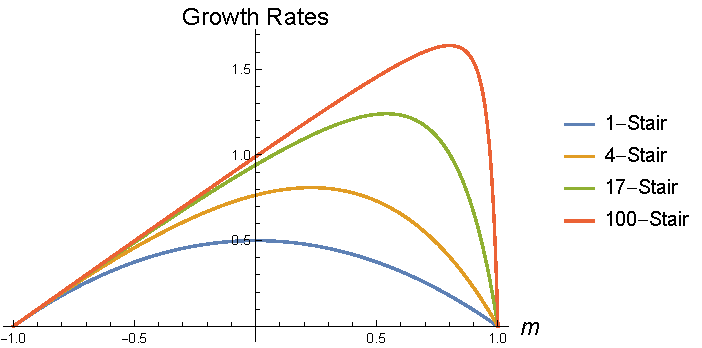
\includegraphics[width=.5\textwidth]{analrates.png}
	\caption{Growth rates for 1-, 4-, 17-, and 100-stairs as a function of slope $m$. As stair length increases, the growth rate asymptotes to the function $\pd{S}{t} = m+1$.}
	\label{fig:growthrates}
\end{figure}

Note that with increasing stair length the growth rate asymptotes to the function $\pd{S}{t} = m+1$. There are two ways to reach this behavior. The first, which matches the order of the current reasoning, is to start with infinite spatial support and take the stair length $n\to\infty$. Alternatively, start with a finite spin chain with length $N$ and periodic boundary conditions, and set the stair length to $N$. Now a single gate acts on site $1,2,3\dots N$, before wrapping around to act at site 1 again. 

The maximal growth rate occurs when the slope is near-maximal, with only a single down step. This corresponds to a slope of $\frac{N-2}{N}$. Then with only a single local minimum in the entropy function, the local minimum moves one site to the right with each gate. Every gate that acts raises the entropy, resulting in an entropy gain of 2 per gate. Of course for a slope of 1, there is still no entropy generation.

If there are 2 down steps, for a slope of $\frac{N-4}{N}$, the entropy generation is almost the same. One local minimum still moves to the right with the leading edge of the staircase. However, once per staircase (once every $N$ gates), one down step is next to the other down step. This results in no entropy growth for that step, for an average entropy gain of $2\frac{N-1}{N}$. Further discussion of the dynamics with near-maximal slope appear in section~\ref{subsub:nearmax}.

This pattern continues as the slope decreases. With $\l$ down steps, the slope is $\frac{N-2\l}{N}$ and the average growth rate is $2\frac{N-\l}{N} = m+1$. At $m = -1$ there is no growth, as expected. At $m=0$, the growth rate is 1, the same as in the brickwork model. With no slope, the steps alternate between up and down, so that half of the gates in any stair are effective, explaining the connection to the brickwork model.

\subsubsection{Near-Maximal Slopes} \emph{} \label{subsub:nearmax}

When the slope is near its largest possible value, so that the entropy increases at nearly every site, it is possible to isolate the behavior of the few down steps. Since gates can only act between a down step and an up step, these ``particles" follow a deterministic behavior and control the entropy growth in the circuit.

Consider a stair with its first gate acting between sites $i$ and $i+1$ and its last gate between $j$ and $j+1$. If there are no down steps in this region, the gate has no effect. 

\subsection{Ergodicity and Stability}\footnote{The following section describes an attempt to calculate steady state correlations. I haven't been successful in doing this yet, but I wanted to write it up in case it proves useful.} \label{sub:erg}\emph{}

A Markov process is one in which the future state depends only on the current state, not the past. Label the states $s_i$ and define $p_{i,t}$ as the probability that the system is in state $s_i$ at time $t$. When there is a constant probability $S_{ij}$ of transitioning from state $j$ to state $i$\footnote{Is this true of all Markov processes?} it is possible to write the transition matrix $S$ such that $p_{i,t+1}= S_{ij}p_{j,t}$. Since the product of the transition matrix and a probability vector gives the probabilities at the next time step, the transition matrix for $t$ time steps is just $S^t$. Under certain conditions\footnote{Figure these out.} the multi-step transition matrix approaches a constant matrix with all columns equal to the same vector $v^*$,
\begin{align}
\lim\limits_{t\to \infty}S^t = S^* = \begin{bmatrix}
\vdots & \vdots &  & \vdots\\
p^* & p^* & \cdots & p^*\\
\vdots & \vdots &  & \vdots\\
\end{bmatrix}.
\end{align}
Then the probability after a long time is the vector $p^*$ for any initial state.

The transition matrix can also be written as $S = 1+T$. The columns of $T$ must sum to 0 to preserve probabilities. From $S^*p^* = p^*,$ it must be true that $Tp^*=0$. This definition provides an easier route to finding $p^*$.

\subsubsection{Stable State in Random Architecture} \emph{} \label{subsub:randstate}

This analysis can be used to find the correlations present in the steady states of staircase architectures. Consider the 1-stair circuit, and enumerate 2-site (3-cut) states by the slope at the 2 sites: $s_1 = d\,d,\; s_2 = d\,u$, etc. Since at every time step there is an equal probability of a gate falling at any site, the transition matrix is the matrix product of single-cut transition matrices $P_{N} = \prod_NP_{1}\otimes$, where the single-cut transition matrix is 
\begin{align}
P_1 = \begin{bmatrix}
1-\frac{1+m}{2}\Gamma & 0      & \frac{1-m}{2}\Gamma & 0\\
\frac{1+m}{2}\Gamma & 1-\Gamma & 0                   & \frac{1-m}{2}\Gamma\\
0                   & \Gamma   & 1-\Gamma            & 0\\
0                   & 0        & \frac{1+m}{2}\Gamma & 1 - \frac{1-m}{2}\Gamma
\end{bmatrix}. \label{eqn:1sitetrans}
\end{align}
The $m$ dependence comes from the possibility of a gate acting on the left or right cut, which depends on the probability of the next slope being up or down.
The equilibrium state is
\begin{align}
v^* = \begin{pmatrix}
\frac{(1-m)^2}{4} \\ 
\frac{1+m}{2}\frac{1-m}{2} \\
\frac{1-m}{2}\frac{1+m}{2} \\
\frac{(1+m)^2}{4}
\end{pmatrix} = \begin{pmatrix}
\frac{1-m}{2} \\ \frac{1+m}{2}
\end{pmatrix} \otimes \begin{pmatrix}
\frac{1-m}{2} \\ \frac{1+m}{2}
\end{pmatrix},
\end{align}
which is uncorrelated, showing that the assumption of lack of correlation (used in equation~\ref{eqn:1sitetrans}) is consistent. Markov's theorem states that if all states are reachable from all other states\footnote{Probably introduce this earlier.} then the system is ergodic. An ergodic system contains only one equilibrium state, so the uncorrelated state is the unique equilibrium state.

\subsubsection{Stable States in Larger Staircases} \emph{} \label{subsub:stairstate}

Finding the stable state in the staircase models is more difficult. Since there are in fact correlations, a transition matrix built using the same method as in equation~\ref{eqn:1sitetrans} would be inexact. One possibility is to assume that the preceding and succeeding slopes are uncorrelated but to consider larger and larger subsystems (instead of the 2 slopes used previously).\footnote{I've made progress on this but haven't finished it.}

\subsection{Numerical Simulation} \emph{}\label{sub:num}

To simulate the entropy growth in infinite spin chains with non-zero slope, we use finite chains with periodic boundary conditions, where one end of the chain is attached to the other with an offset. The spin chains are initialized with a highly correlated\footnote{A next step is to fix the initialization so that the states start uncorrelated.} entropy function with the given slope. Since larger gates will generate different correlation, growth rates are calculated for only the latter part of the simulation, ensuring that the entropy is in its equilibrium state.

\subsubsection{Measuring Growth Rates} \emph{} \label{subsub:growthrates}

Growth rates for stairs of various lengths are shown in figure~\ref{fig:compareRates}. As length increases, the growth rate follows the same pattern as predicted, increasing with the maximum moving right. 
\begin{figure}
	\centering
	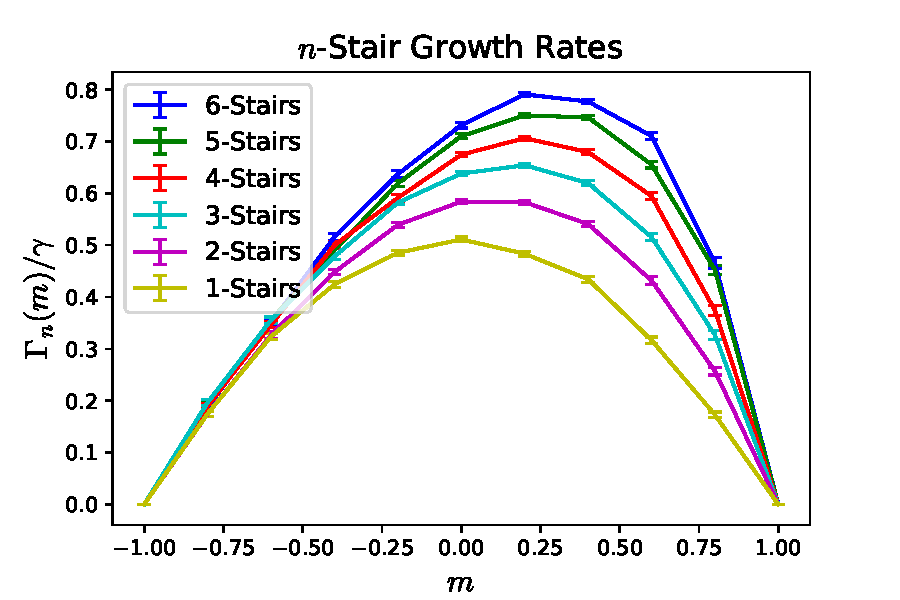
\includegraphics[width=.5\textwidth]{compareRates.pdf}
	\caption{\textbf{Growth rates for different length stairs.} All growth rates were calculated using a 100-site spin chain with offset periodic boundary conditions. Rates were calculated from the application of 100,000 gates, averaged over the last 80\% of the gates in order to build up correlations.}
	\label{fig:compareRates}
\end{figure}

For 1-stairs (the random architecture), the measured growth rate is slightly larger than predicted, seen in figure~\ref{fig:1stairRates}.
\begin{figure}
	\centering
	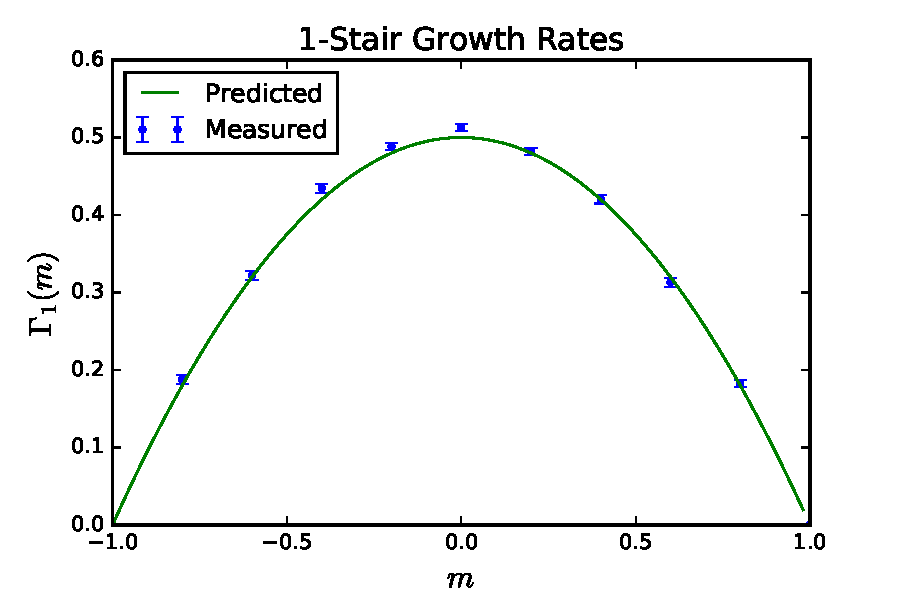
\includegraphics[width=.5\textwidth]{1stairRates.pdf}
	\caption{\textbf{Measured and analytic growth rates} for the 1-stair architecture. Note that the measured rate is slightly higher. Since the assumption of un-correlation is exact for 1-stairs, this difference is assumed to be due to second order derivatives in the slope and finite length effects.}
	\label{fig:1stairRates}
\end{figure}
There are two main differences between the analytic and measured setups. For the analytic result, the chain is infinite and the entropy function is assumed to be linear and uncorrelated. Since the assumption of un-correlation is exact for 1-stairs, this difference is assumed to be due to second order derivatives in the slope and finite length effects.

Stairs of length greater than 1 do however generate correlations. Figure~\ref{fig:6stairRates} shows the growth rates for 6-stairs. 
\begin{figure}
	\centering
	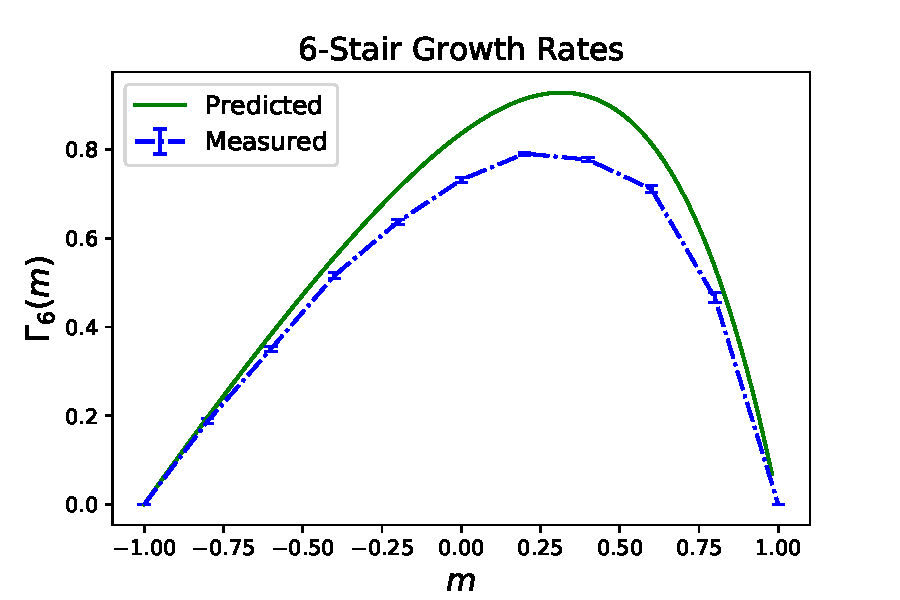
\includegraphics[width=.5\textwidth]{6stairRates.pdf}
	\caption{\textbf{Measured and predicted growth rates} for the 6-stair architecture. The measured rate is now lower than predicted, implying that the correlations built up by the stairs act to lower their entropy production.}
	\label{fig:6stairRates}
\end{figure}
The notable difference in growth rate here is probably due to correlations created by the 6-stairs. Hopefully reasoning similar to that in section~\ref{sub:erg} will be able to predict the correlation so that its effect, at least to first order, can be calculated. This would allow a much closer approximation than that in figure~\ref{fig:6stairRates}

\subsubsection{Measuring Correlations} \emph{} \label{subsub:correlations}

The first step in understanding the difference between predicted and measured behavior is understanding the correlations introduced by the gates. Figure~\ref{fig:stairCorrel} shows the initial and final correlations for the 1- and 3-stair circuits. Both curves were created by averaging over the correlation in the second half of a 10,000 step run, averaged over 10 runs.
\begin{figure}
	\centering
	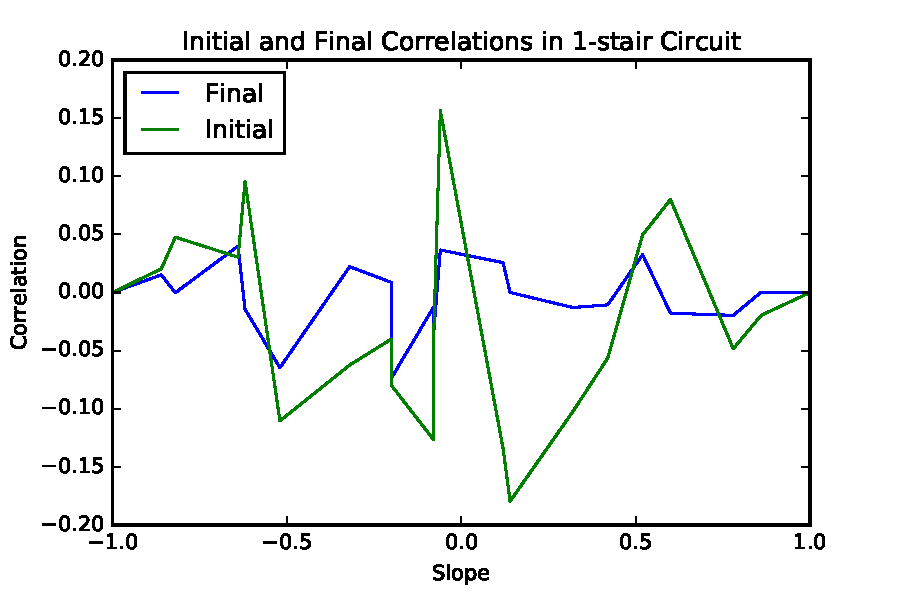
\includegraphics[width=.495\textwidth]{1stairCorrel}
	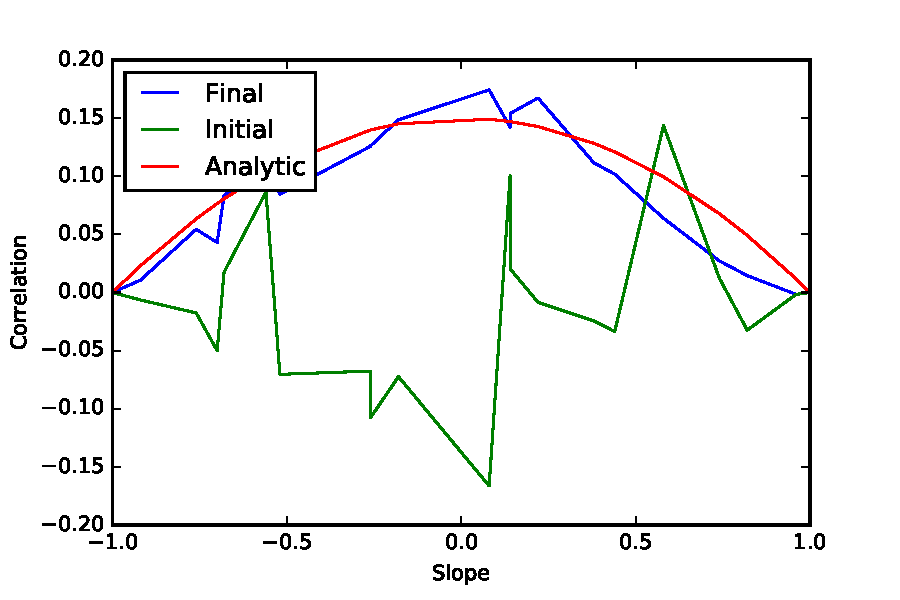
\includegraphics[width=.495\textwidth]{3stairCorrel}
	\caption{\textbf{Correlations created by 1- and 3-stair circuits.} The initial correlation curve shows that because of the initialization procedure the slope-0 state is perfectly anti-correlated. However, the correlation quickly equilibrates (see figure~\ref{fig:corrgrowth}). The 3-stair circuit reaches a more highly-correlated state than the 1-stair circuit.}
	\label{fig:stairCorrel}
\end{figure}
The 3-stair circuit indeed generates more correlation than the 1-stair circuit. 

Although the initial state is highly anticorrelated, the evolution of the circuit quickly removes this correlation, as shown in figure~\ref{fig:corrgrowth}.
\begin{figure}
	\centering
	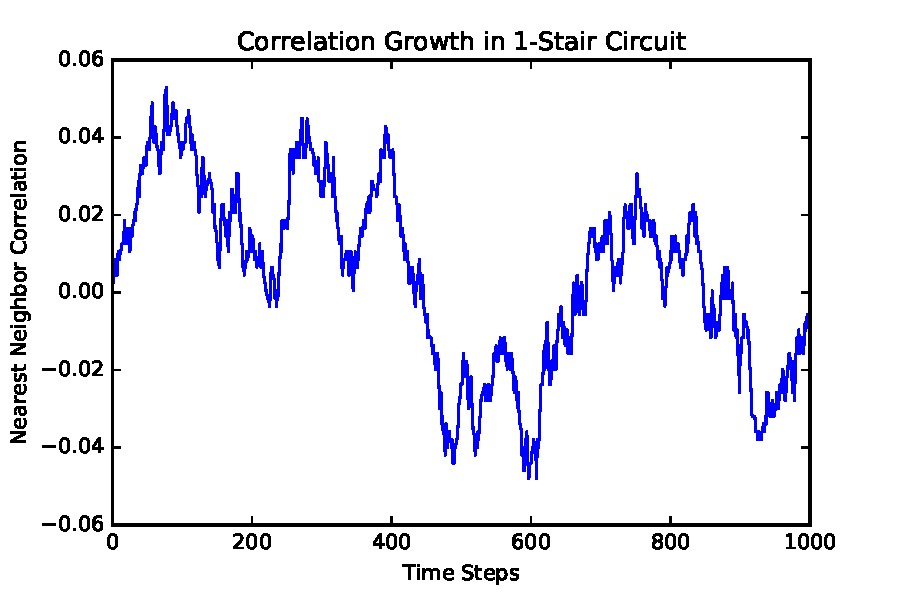
\includegraphics[width=.5\textwidth]{corrgrowth.pdf}
	\caption{\textbf{Correlation Growth for 0 slope.} Although the state starts out artificially anticorrelated, the correlation equilibrates after 400-600 time steps.}
	\label{fig:corrgrowth}
\end{figure}
The correlation saturates after 400-600 time steps, meaning the correlation of the initial state is not as important as the overall slope. For 1-stairs the correlation should asymptote to 0, as it appears to do. An interesting next step would be a way to analytically predict the correlation built by each circuit.
%\printbibliography

\end{document}
